% Options for packages loaded elsewhere
\PassOptionsToPackage{unicode}{hyperref}
\PassOptionsToPackage{hyphens}{url}
\documentclass[
]{article}
\usepackage{xcolor}
\usepackage[margin=1in]{geometry}
\usepackage{amsmath,amssymb}
\setcounter{secnumdepth}{-\maxdimen} % remove section numbering
\usepackage{iftex}
\ifPDFTeX
  \usepackage[T1]{fontenc}
  \usepackage[utf8]{inputenc}
  \usepackage{textcomp} % provide euro and other symbols
\else % if luatex or xetex
  \usepackage{unicode-math} % this also loads fontspec
  \defaultfontfeatures{Scale=MatchLowercase}
  \defaultfontfeatures[\rmfamily]{Ligatures=TeX,Scale=1}
\fi
\usepackage{lmodern}
\ifPDFTeX\else
  % xetex/luatex font selection
\fi
% Use upquote if available, for straight quotes in verbatim environments
\IfFileExists{upquote.sty}{\usepackage{upquote}}{}
\IfFileExists{microtype.sty}{% use microtype if available
  \usepackage[]{microtype}
  \UseMicrotypeSet[protrusion]{basicmath} % disable protrusion for tt fonts
}{}
\makeatletter
\@ifundefined{KOMAClassName}{% if non-KOMA class
  \IfFileExists{parskip.sty}{%
    \usepackage{parskip}
  }{% else
    \setlength{\parindent}{0pt}
    \setlength{\parskip}{6pt plus 2pt minus 1pt}}
}{% if KOMA class
  \KOMAoptions{parskip=half}}
\makeatother
\usepackage{color}
\usepackage{fancyvrb}
\newcommand{\VerbBar}{|}
\newcommand{\VERB}{\Verb[commandchars=\\\{\}]}
\DefineVerbatimEnvironment{Highlighting}{Verbatim}{commandchars=\\\{\}}
% Add ',fontsize=\small' for more characters per line
\usepackage{framed}
\definecolor{shadecolor}{RGB}{248,248,248}
\newenvironment{Shaded}{\begin{snugshade}}{\end{snugshade}}
\newcommand{\AlertTok}[1]{\textcolor[rgb]{0.94,0.16,0.16}{#1}}
\newcommand{\AnnotationTok}[1]{\textcolor[rgb]{0.56,0.35,0.01}{\textbf{\textit{#1}}}}
\newcommand{\AttributeTok}[1]{\textcolor[rgb]{0.13,0.29,0.53}{#1}}
\newcommand{\BaseNTok}[1]{\textcolor[rgb]{0.00,0.00,0.81}{#1}}
\newcommand{\BuiltInTok}[1]{#1}
\newcommand{\CharTok}[1]{\textcolor[rgb]{0.31,0.60,0.02}{#1}}
\newcommand{\CommentTok}[1]{\textcolor[rgb]{0.56,0.35,0.01}{\textit{#1}}}
\newcommand{\CommentVarTok}[1]{\textcolor[rgb]{0.56,0.35,0.01}{\textbf{\textit{#1}}}}
\newcommand{\ConstantTok}[1]{\textcolor[rgb]{0.56,0.35,0.01}{#1}}
\newcommand{\ControlFlowTok}[1]{\textcolor[rgb]{0.13,0.29,0.53}{\textbf{#1}}}
\newcommand{\DataTypeTok}[1]{\textcolor[rgb]{0.13,0.29,0.53}{#1}}
\newcommand{\DecValTok}[1]{\textcolor[rgb]{0.00,0.00,0.81}{#1}}
\newcommand{\DocumentationTok}[1]{\textcolor[rgb]{0.56,0.35,0.01}{\textbf{\textit{#1}}}}
\newcommand{\ErrorTok}[1]{\textcolor[rgb]{0.64,0.00,0.00}{\textbf{#1}}}
\newcommand{\ExtensionTok}[1]{#1}
\newcommand{\FloatTok}[1]{\textcolor[rgb]{0.00,0.00,0.81}{#1}}
\newcommand{\FunctionTok}[1]{\textcolor[rgb]{0.13,0.29,0.53}{\textbf{#1}}}
\newcommand{\ImportTok}[1]{#1}
\newcommand{\InformationTok}[1]{\textcolor[rgb]{0.56,0.35,0.01}{\textbf{\textit{#1}}}}
\newcommand{\KeywordTok}[1]{\textcolor[rgb]{0.13,0.29,0.53}{\textbf{#1}}}
\newcommand{\NormalTok}[1]{#1}
\newcommand{\OperatorTok}[1]{\textcolor[rgb]{0.81,0.36,0.00}{\textbf{#1}}}
\newcommand{\OtherTok}[1]{\textcolor[rgb]{0.56,0.35,0.01}{#1}}
\newcommand{\PreprocessorTok}[1]{\textcolor[rgb]{0.56,0.35,0.01}{\textit{#1}}}
\newcommand{\RegionMarkerTok}[1]{#1}
\newcommand{\SpecialCharTok}[1]{\textcolor[rgb]{0.81,0.36,0.00}{\textbf{#1}}}
\newcommand{\SpecialStringTok}[1]{\textcolor[rgb]{0.31,0.60,0.02}{#1}}
\newcommand{\StringTok}[1]{\textcolor[rgb]{0.31,0.60,0.02}{#1}}
\newcommand{\VariableTok}[1]{\textcolor[rgb]{0.00,0.00,0.00}{#1}}
\newcommand{\VerbatimStringTok}[1]{\textcolor[rgb]{0.31,0.60,0.02}{#1}}
\newcommand{\WarningTok}[1]{\textcolor[rgb]{0.56,0.35,0.01}{\textbf{\textit{#1}}}}
\usepackage{longtable,booktabs,array}
\usepackage{calc} % for calculating minipage widths
% Correct order of tables after \paragraph or \subparagraph
\usepackage{etoolbox}
\makeatletter
\patchcmd\longtable{\par}{\if@noskipsec\mbox{}\fi\par}{}{}
\makeatother
% Allow footnotes in longtable head/foot
\IfFileExists{footnotehyper.sty}{\usepackage{footnotehyper}}{\usepackage{footnote}}
\makesavenoteenv{longtable}
\usepackage{graphicx}
\makeatletter
\newsavebox\pandoc@box
\newcommand*\pandocbounded[1]{% scales image to fit in text height/width
  \sbox\pandoc@box{#1}%
  \Gscale@div\@tempa{\textheight}{\dimexpr\ht\pandoc@box+\dp\pandoc@box\relax}%
  \Gscale@div\@tempb{\linewidth}{\wd\pandoc@box}%
  \ifdim\@tempb\p@<\@tempa\p@\let\@tempa\@tempb\fi% select the smaller of both
  \ifdim\@tempa\p@<\p@\scalebox{\@tempa}{\usebox\pandoc@box}%
  \else\usebox{\pandoc@box}%
  \fi%
}
% Set default figure placement to htbp
\def\fps@figure{htbp}
\makeatother
% definitions for citeproc citations
\NewDocumentCommand\citeproctext{}{}
\NewDocumentCommand\citeproc{mm}{%
  \begingroup\def\citeproctext{#2}\cite{#1}\endgroup}
\makeatletter
 % allow citations to break across lines
 \let\@cite@ofmt\@firstofone
 % avoid brackets around text for \cite:
 \def\@biblabel#1{}
 \def\@cite#1#2{{#1\if@tempswa , #2\fi}}
\makeatother
\newlength{\cslhangindent}
\setlength{\cslhangindent}{1.5em}
\newlength{\csllabelwidth}
\setlength{\csllabelwidth}{3em}
\newenvironment{CSLReferences}[2] % #1 hanging-indent, #2 entry-spacing
 {\begin{list}{}{%
  \setlength{\itemindent}{0pt}
  \setlength{\leftmargin}{0pt}
  \setlength{\parsep}{0pt}
  % turn on hanging indent if param 1 is 1
  \ifodd #1
   \setlength{\leftmargin}{\cslhangindent}
   \setlength{\itemindent}{-1\cslhangindent}
  \fi
  % set entry spacing
  \setlength{\itemsep}{#2\baselineskip}}}
 {\end{list}}
\usepackage{calc}
\newcommand{\CSLBlock}[1]{\hfill\break\parbox[t]{\linewidth}{\strut\ignorespaces#1\strut}}
\newcommand{\CSLLeftMargin}[1]{\parbox[t]{\csllabelwidth}{\strut#1\strut}}
\newcommand{\CSLRightInline}[1]{\parbox[t]{\linewidth - \csllabelwidth}{\strut#1\strut}}
\newcommand{\CSLIndent}[1]{\hspace{\cslhangindent}#1}
\setlength{\emergencystretch}{3em} % prevent overfull lines
\providecommand{\tightlist}{%
  \setlength{\itemsep}{0pt}\setlength{\parskip}{0pt}}
\usepackage{bookmark}
\IfFileExists{xurl.sty}{\usepackage{xurl}}{} % add URL line breaks if available
\urlstyle{same}
\hypersetup{
  pdftitle={REDD+ Feasability Assessment Review},
  hidelinks,
  pdfcreator={LaTeX via pandoc}}

\title{REDD+ Feasability Assessment Review}
\usepackage{etoolbox}
\makeatletter
\providecommand{\subtitle}[1]{% add subtitle to \maketitle
  \apptocmd{\@title}{\par {\large #1 \par}}{}{}
}
\makeatother
\subtitle{Review of emissions estimates \& activity data used in the
RSPB Gola feasibility assessment}
\author{}
\date{\vspace{-2.5em}2024-12-23}

\begin{document}
\maketitle

\subsection{Summary}\label{summary}

This initial review of the VT0007 estimates and the RSPB REDD+
feasibility study aims to provide a preliminary comparison of forest
area estimates and methodologies. It highlights some discrepancies in
the results, which may reflect differences in the methods and
assumptions used. However, this review is an early effort and remains
open for correction or improvement, with the understanding that previous
methods may yet provide the more accurate representation. Further
analysis and development were paused pending decisions from the project
leaders regarding the allocation of billed hours.

\begin{enumerate}
\def\labelenumi{\arabic{enumi}.}
\item
  \textbf{Forest Area Estimates:}

  \begin{itemize}
  \item
    Our analysis showed:

    \begin{itemize}
    \item
      \textbf{2014}: 9,332,083 ha
    \item
      \textbf{2019}: 8,851,256 ha
    \item
      \textbf{2024}: 9,297,764 ha
    \end{itemize}
  \item
    These values differ from the report, particularly for \textbf{Gola
    NP} in 2013 (88,289.72 ha), suggesting possible differences in data
    or methods.
  \end{itemize}
\item
  \textbf{Deforestation Rates:}

  \begin{itemize}
  \tightlist
  \item
    The reported deforestation rates (Norman: \textbf{0.17\%}, Tonglay:
    \textbf{0.21\%}) seem to differ from our estimates, possibly due to
    varying data sources or assumptions.
  \end{itemize}
\item
  \textbf{REDD+ Scenarios:}

  \begin{itemize}
  \tightlist
  \item
    The reported \textbf{REDD+} forest area for \textbf{Gola NP} was
    100\%, while our figures were slightly lower, potentially due to
    different approaches in spatial data handling.
  \end{itemize}
\item
  \textbf{Methodology:}

  \begin{itemize}
  \tightlist
  \item
    We used raster transformations to ensure consistency, which might
    explain some of the differences. Exploring these methodologies could
    help clarify discrepancies.
  \end{itemize}
\item
  \textbf{Next Steps:}

  \begin{itemize}
  \tightlist
  \item
    We suggest revisiting the methods and data sources used in both
    analyses to better understand the differences and improve the
    consistency of the results.
  \end{itemize}
\end{enumerate}

These points reflect initial observations, and further investigation may
be needed to fully align both analyses.

\pandocbounded{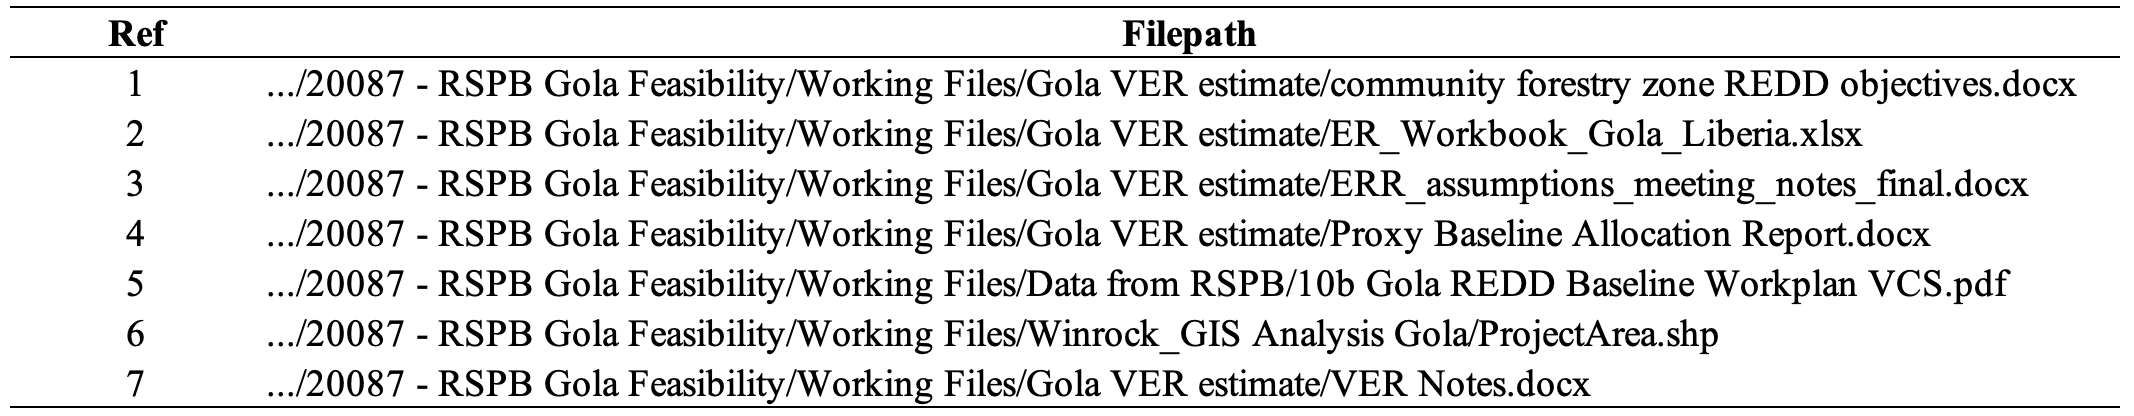
\includegraphics[keepaspectratio]{images/Table 1 Project files reviewed.png}}

\subparagraph{Table 1: Project files reviewed in this
assessment}\label{table-1-project-files-reviewed-in-this-assessment}

\emph{Import AOI:}

\begin{Shaded}
\begin{Highlighting}[]
\FunctionTok{set.seed}\NormalTok{(}\DecValTok{77777}\NormalTok{)}
\CommentTok{\# Import project area aoi}
\NormalTok{aoi }\OtherTok{=}\NormalTok{ sf}\SpecialCharTok{::}\FunctionTok{read\_sf}\NormalTok{(}\StringTok{".../Winrock\_GIS Analysis Gola/ProjectArea.shp"}\NormalTok{) }
\NormalTok{aoi }\OtherTok{=}\NormalTok{ aoi }\SpecialCharTok{|\textgreater{}}
\NormalTok{  sf}\SpecialCharTok{::}\FunctionTok{st\_cast}\NormalTok{(}\StringTok{"POLYGON"}\NormalTok{) }\SpecialCharTok{|\textgreater{}}
\NormalTok{  sf}\SpecialCharTok{::}\FunctionTok{st\_cast}\NormalTok{(}\StringTok{"MULTIPOLYGON"}\NormalTok{) }\SpecialCharTok{|\textgreater{}}
\NormalTok{  dplyr}\SpecialCharTok{::}\FunctionTok{filter}\NormalTok{(}
\NormalTok{    NAME   }\SpecialCharTok{==} \StringTok{"Gola Forest National Park"} \SpecialCharTok{|} 
\NormalTok{      NAME }\SpecialCharTok{==} \StringTok{"Tonglay"} \SpecialCharTok{|}
\NormalTok{      NAME }\SpecialCharTok{==} \StringTok{"Normon"}\NormalTok{)}
\CommentTok{\# Import national area aoi}
\NormalTok{query }\OtherTok{=}\NormalTok{ osmdata}\SpecialCharTok{::}\FunctionTok{opq}\NormalTok{(}\StringTok{"Liberia"}\NormalTok{) }\SpecialCharTok{|\textgreater{}} \CommentTok{\# opq = overpass query}
\NormalTok{  osmdata}\SpecialCharTok{::}\FunctionTok{add\_osm\_feature}\NormalTok{(}\AttributeTok{key =} \StringTok{"boundary"}\NormalTok{, }\AttributeTok{value =} \StringTok{"administrative"}\NormalTok{) }\SpecialCharTok{|\textgreater{}}
\NormalTok{  osmdata}\SpecialCharTok{::}\FunctionTok{osmdata\_sf}\NormalTok{()}
\NormalTok{boundaries }\OtherTok{=}\NormalTok{ query}\SpecialCharTok{$}\NormalTok{osm\_multipolygons}
\NormalTok{country  }\OtherTok{=}\NormalTok{ boundaries }\SpecialCharTok{|\textgreater{}}
\NormalTok{  dplyr}\SpecialCharTok{::}\FunctionTok{filter}\NormalTok{(admin\_level }\SpecialCharTok{==} \StringTok{"2"}\NormalTok{, name }\SpecialCharTok{==} \StringTok{"Liberia"}\NormalTok{) }\SpecialCharTok{|\textgreater{}}
\NormalTok{  dplyr}\SpecialCharTok{::}\FunctionTok{select}\NormalTok{(name, admin\_level, geometry) }\SpecialCharTok{|\textgreater{}}
\NormalTok{  sf}\SpecialCharTok{::}\FunctionTok{st\_cast}\NormalTok{() }\SpecialCharTok{|\textgreater{}} 
\NormalTok{  sf}\SpecialCharTok{::}\FunctionTok{st\_transform}\NormalTok{(}\DecValTok{4326}\NormalTok{)}
\NormalTok{sf}\SpecialCharTok{::}\FunctionTok{st\_write}\NormalTok{(country, }\StringTok{"./data/aoi/liberia\_boundary\_national.shp"}\NormalTok{, }\AttributeTok{delete\_layer=}\NormalTok{T)}
\end{Highlighting}
\end{Shaded}

\begin{Shaded}
\begin{Highlighting}[]
\NormalTok{tmap}\SpecialCharTok{::}\FunctionTok{tmap\_mode}\NormalTok{(}\StringTok{"plot"}\NormalTok{)}
\CommentTok{\# zoom = 11 = 1:150,000 scale {-} https://wiki.openstreetmap.org/wiki/Zoom\_levels}
\NormalTok{basemap\_aoi }\OtherTok{=}\NormalTok{ maptiles}\SpecialCharTok{::}\FunctionTok{get\_tiles}\NormalTok{(}
\NormalTok{  bbox\_aoi\_2, }
  \AttributeTok{zoom      =} \DecValTok{10}\NormalTok{, }
  \AttributeTok{crop      =}\NormalTok{ T,}
  \AttributeTok{provider  =} \StringTok{"Esri.NatGeoWorldMap"}
\NormalTok{  )}

\NormalTok{basemap\_country }\OtherTok{=}\NormalTok{ maptiles}\SpecialCharTok{::}\FunctionTok{get\_tiles}\NormalTok{(}
\NormalTok{  bbox\_country\_2, }
  \AttributeTok{zoom      =} \DecValTok{8}\NormalTok{, }
  \AttributeTok{crop      =}\NormalTok{ T,}
  \AttributeTok{provider  =} \StringTok{"Esri.NatGeoWorldMap"}
\NormalTok{  )}

\NormalTok{tmap}\SpecialCharTok{::}\FunctionTok{tm\_shape}\NormalTok{(bbox\_aoi) }\SpecialCharTok{+}\NormalTok{ tmap}\SpecialCharTok{::}\FunctionTok{tm\_borders}\NormalTok{(}\AttributeTok{lwd =} \FloatTok{0.0}\NormalTok{) }\SpecialCharTok{+}
\NormalTok{  tmap}\SpecialCharTok{::}\FunctionTok{tm\_shape}\NormalTok{(basemap\_aoi) }\SpecialCharTok{+}\NormalTok{ tmap}\SpecialCharTok{::}\FunctionTok{tm\_rgb}\NormalTok{() }\SpecialCharTok{+} 
\NormalTok{  tmap}\SpecialCharTok{::}\FunctionTok{tm\_shape}\NormalTok{(aoi) }\SpecialCharTok{+}\NormalTok{ tmap}\SpecialCharTok{::}\FunctionTok{tm\_borders}\NormalTok{(}\AttributeTok{lwd =} \DecValTok{2}\NormalTok{, }\AttributeTok{col =} \StringTok{"red"}\NormalTok{) }\SpecialCharTok{+}
\NormalTok{  tmap}\SpecialCharTok{::}\FunctionTok{tm\_text}\NormalTok{(}\StringTok{"NAME"}\NormalTok{, }\AttributeTok{just =} \StringTok{"center"}\NormalTok{, }\AttributeTok{col=}\StringTok{"black"}\NormalTok{, }\AttributeTok{size=}\FloatTok{0.6}\NormalTok{) }\SpecialCharTok{+}
\NormalTok{  tmap}\SpecialCharTok{::}\FunctionTok{tm\_graticules}\NormalTok{(}\AttributeTok{lines=}\NormalTok{T,}\AttributeTok{labels.rot=}\FunctionTok{c}\NormalTok{(}\DecValTok{0}\NormalTok{,}\DecValTok{90}\NormalTok{),}\AttributeTok{lwd=}\FloatTok{0.2}\NormalTok{) }\SpecialCharTok{+}
\NormalTok{  tmap}\SpecialCharTok{::}\FunctionTok{tm\_credits}\NormalTok{(}\StringTok{"EPSG:32629"}\NormalTok{, }\AttributeTok{position =} \FunctionTok{c}\NormalTok{(}\StringTok{"left"}\NormalTok{, }\StringTok{"bottom"}\NormalTok{)) }\SpecialCharTok{+}
\NormalTok{  tmap}\SpecialCharTok{::}\FunctionTok{tm\_scale\_bar}\NormalTok{(}\AttributeTok{position =} \FunctionTok{c}\NormalTok{(}\StringTok{"RIGHT"}\NormalTok{, }\StringTok{"BOTTOM"}\NormalTok{), }\AttributeTok{text.size =}\NormalTok{ .}\DecValTok{5}\NormalTok{) }\SpecialCharTok{+} 
\NormalTok{  tmap}\SpecialCharTok{::}\FunctionTok{tm\_compass}\NormalTok{(}\AttributeTok{color.dark =} \StringTok{"gray60"}\NormalTok{, }\AttributeTok{text.color =} \StringTok{"gray60"}\NormalTok{, }\AttributeTok{position =} \FunctionTok{c}\NormalTok{(}\StringTok{"left"}\NormalTok{, }\StringTok{"top"}\NormalTok{)) }\OtherTok{{-}\textgreater{}}\NormalTok{ tm1}

\NormalTok{tmap}\SpecialCharTok{::}\FunctionTok{tm\_shape}\NormalTok{(bbox\_country) }\SpecialCharTok{+}\NormalTok{ tmap}\SpecialCharTok{::}\FunctionTok{tm\_borders}\NormalTok{(}\AttributeTok{lwd =} \FloatTok{0.0}\NormalTok{) }\SpecialCharTok{+}
\NormalTok{  tmap}\SpecialCharTok{::}\FunctionTok{tm\_shape}\NormalTok{(basemap\_country) }\SpecialCharTok{+}\NormalTok{ tmap}\SpecialCharTok{::}\FunctionTok{tm\_rgb}\NormalTok{() }\SpecialCharTok{+} 
\NormalTok{  tmap}\SpecialCharTok{::}\FunctionTok{tm\_shape}\NormalTok{(country) }\SpecialCharTok{+}\NormalTok{ tmap}\SpecialCharTok{::}\FunctionTok{tm\_borders}\NormalTok{(}\AttributeTok{col =} \StringTok{"blue"}\NormalTok{, }\AttributeTok{lwd =} \DecValTok{2}\NormalTok{) }\SpecialCharTok{+}
\NormalTok{  tmap}\SpecialCharTok{::}\FunctionTok{tm\_shape}\NormalTok{(aoi) }\SpecialCharTok{+}\NormalTok{ tmap}\SpecialCharTok{::}\FunctionTok{tm\_borders}\NormalTok{(}\AttributeTok{col =} \StringTok{"red"}\NormalTok{, }\AttributeTok{lwd =} \DecValTok{2}\NormalTok{) }\SpecialCharTok{+}
\NormalTok{  tmap}\SpecialCharTok{::}\FunctionTok{tm\_graticules}\NormalTok{(}\AttributeTok{lines=}\NormalTok{T,}\AttributeTok{labels.rot=}\FunctionTok{c}\NormalTok{(}\DecValTok{0}\NormalTok{,}\DecValTok{90}\NormalTok{),}\AttributeTok{lwd=}\FloatTok{0.2}\NormalTok{) }\SpecialCharTok{+}
\NormalTok{  tmap}\SpecialCharTok{::}\FunctionTok{tm\_credits}\NormalTok{(}\StringTok{"EPSG:4326"}\NormalTok{, }\AttributeTok{position =} \FunctionTok{c}\NormalTok{(}\StringTok{"left"}\NormalTok{, }\StringTok{"bottom"}\NormalTok{)) }\SpecialCharTok{+}
\NormalTok{  tmap}\SpecialCharTok{::}\FunctionTok{tm\_scale\_bar}\NormalTok{(}\AttributeTok{position =} \FunctionTok{c}\NormalTok{(}\StringTok{"RIGHT"}\NormalTok{, }\StringTok{"BOTTOM"}\NormalTok{), }\AttributeTok{text.size =}\NormalTok{ .}\DecValTok{5}\NormalTok{) }\SpecialCharTok{+} 
\NormalTok{  tmap}\SpecialCharTok{::}\FunctionTok{tm\_compass}\NormalTok{(}\AttributeTok{color.dark =} \StringTok{"gray60"}\NormalTok{, }\AttributeTok{text.color =} \StringTok{"gray60"}\NormalTok{, }\AttributeTok{position =} \FunctionTok{c}\NormalTok{(}\StringTok{"left"}\NormalTok{, }\StringTok{"top"}\NormalTok{)) }\OtherTok{{-}\textgreater{}}\NormalTok{ tm2}
                   
\NormalTok{tmap}\SpecialCharTok{::}\FunctionTok{tmap\_save}\NormalTok{(tm1, }\StringTok{"./data/site\_maps/site\_map.png"}\NormalTok{, }\AttributeTok{height=}\DecValTok{10000}\NormalTok{, }\AttributeTok{asp=}\DecValTok{0}\NormalTok{, }\AttributeTok{dpi=}\DecValTok{2400}\NormalTok{)}
\NormalTok{tmap}\SpecialCharTok{::}\FunctionTok{tmap\_save}\NormalTok{(tm2, }\StringTok{"./data/site\_maps/locator\_map.png"}\NormalTok{, }\AttributeTok{height=}\DecValTok{10000}\NormalTok{, }\AttributeTok{asp=}\DecValTok{0}\NormalTok{, }\AttributeTok{dpi=}\DecValTok{2400}\NormalTok{)}
\NormalTok{tmap}\SpecialCharTok{::}\FunctionTok{tmap\_arrange}\NormalTok{(tm1, tm2, }\AttributeTok{ncol=}\DecValTok{2}\NormalTok{)}
\end{Highlighting}
\end{Shaded}

\begin{Shaded}
\begin{Highlighting}[]
\NormalTok{knitr}\SpecialCharTok{::}\FunctionTok{include\_graphics}\NormalTok{(}\FunctionTok{c}\NormalTok{(}\StringTok{"\textasciitilde{}/repos/rspb{-}redd{-}feasability/data/site\_maps/site\_map.png"}\NormalTok{,}
                          \StringTok{"\textasciitilde{}/repos/rspb{-}redd{-}feasability/data/site\_maps/locator\_map.png"}\NormalTok{))}
\end{Highlighting}
\end{Shaded}

\includegraphics[width=0.5\linewidth]{data/site_maps/site_map}
\includegraphics[width=0.5\linewidth]{data/site_maps/locator_map}

\subsection{Area check}\label{area-check}

In Liberia, the official definition of forest land is provided by the
Forestry Development Authority (Liberia 2019), including areas of land
that meet the following criteria:

\begin{itemize}
\tightlist
\item
  Canopy cover of minimum 30\%;
\item
  Canopy height of minimum 5m or the capacity to reach it;
\item
  Covering a minimum of 1 hectare of land.
\end{itemize}

\begin{Shaded}
\begin{Highlighting}[]
\NormalTok{aoi}\SpecialCharTok{$}\NormalTok{area\_m2 }\OtherTok{=} \FunctionTok{round}\NormalTok{(}\FunctionTok{as.numeric}\NormalTok{(sf}\SpecialCharTok{::}\FunctionTok{st\_area}\NormalTok{(aoi) }\SpecialCharTok{*} \FloatTok{0.0001}\NormalTok{, }\DecValTok{4}\NormalTok{))}
\NormalTok{aoi\_select }\OtherTok{=}\NormalTok{ aoi }\SpecialCharTok{|\textgreater{}}
\NormalTok{  dplyr}\SpecialCharTok{::}\FunctionTok{select}\NormalTok{(NAME, DESIG, Areahav2, area\_m2) }\SpecialCharTok{|\textgreater{}}
\NormalTok{  dplyr}\SpecialCharTok{::}\FunctionTok{filter}\NormalTok{(}
\NormalTok{    NAME }\SpecialCharTok{==} \StringTok{"Gola Forest National Park"} \SpecialCharTok{|} 
\NormalTok{      NAME }\SpecialCharTok{==} \StringTok{"Normon"}  \SpecialCharTok{|} 
\NormalTok{      NAME }\SpecialCharTok{==} \StringTok{"Tonglay"}\NormalTok{) }\SpecialCharTok{|\textgreater{}}
\NormalTok{  sf}\SpecialCharTok{::}\FunctionTok{st\_drop\_geometry}\NormalTok{() }\SpecialCharTok{|\textgreater{}}
\NormalTok{  janitor}\SpecialCharTok{::}\FunctionTok{adorn\_totals}\NormalTok{() }
\NormalTok{sf}\SpecialCharTok{::}\FunctionTok{st\_transform}\NormalTok{(aoi, }\DecValTok{4326}\NormalTok{)  }
\end{Highlighting}
\end{Shaded}

\begin{longtable}[]{@{}
  >{\raggedleft\arraybackslash}p{(\linewidth - 60\tabcolsep) * \real{0.0198}}
  >{\raggedright\arraybackslash}p{(\linewidth - 60\tabcolsep) * \real{0.0198}}
  >{\raggedright\arraybackslash}p{(\linewidth - 60\tabcolsep) * \real{0.0516}}
  >{\raggedright\arraybackslash}p{(\linewidth - 60\tabcolsep) * \real{0.0516}}
  >{\raggedright\arraybackslash}p{(\linewidth - 60\tabcolsep) * \real{0.0337}}
  >{\raggedright\arraybackslash}p{(\linewidth - 60\tabcolsep) * \real{0.0218}}
  >{\raggedright\arraybackslash}p{(\linewidth - 60\tabcolsep) * \real{0.0258}}
  >{\raggedright\arraybackslash}p{(\linewidth - 60\tabcolsep) * \real{0.0298}}
  >{\raggedright\arraybackslash}p{(\linewidth - 60\tabcolsep) * \real{0.0139}}
  >{\raggedleft\arraybackslash}p{(\linewidth - 60\tabcolsep) * \real{0.0218}}
  >{\raggedleft\arraybackslash}p{(\linewidth - 60\tabcolsep) * \real{0.0218}}
  >{\raggedleft\arraybackslash}p{(\linewidth - 60\tabcolsep) * \real{0.0198}}
  >{\raggedleft\arraybackslash}p{(\linewidth - 60\tabcolsep) * \real{0.0218}}
  >{\raggedright\arraybackslash}p{(\linewidth - 60\tabcolsep) * \real{0.0218}}
  >{\raggedleft\arraybackslash}p{(\linewidth - 60\tabcolsep) * \real{0.0198}}
  >{\raggedright\arraybackslash}p{(\linewidth - 60\tabcolsep) * \real{0.0774}}
  >{\raggedright\arraybackslash}p{(\linewidth - 60\tabcolsep) * \real{0.1310}}
  >{\raggedright\arraybackslash}p{(\linewidth - 60\tabcolsep) * \real{0.0258}}
  >{\raggedright\arraybackslash}p{(\linewidth - 60\tabcolsep) * \real{0.0298}}
  >{\raggedleft\arraybackslash}p{(\linewidth - 60\tabcolsep) * \real{0.0218}}
  >{\raggedright\arraybackslash}p{(\linewidth - 60\tabcolsep) * \real{0.0159}}
  >{\raggedright\arraybackslash}p{(\linewidth - 60\tabcolsep) * \real{0.0218}}
  >{\raggedright\arraybackslash}p{(\linewidth - 60\tabcolsep) * \real{0.0099}}
  >{\raggedright\arraybackslash}p{(\linewidth - 60\tabcolsep) * \real{0.0655}}
  >{\raggedright\arraybackslash}p{(\linewidth - 60\tabcolsep) * \real{0.0456}}
  >{\raggedleft\arraybackslash}p{(\linewidth - 60\tabcolsep) * \real{0.0218}}
  >{\raggedleft\arraybackslash}p{(\linewidth - 60\tabcolsep) * \real{0.0218}}
  >{\raggedleft\arraybackslash}p{(\linewidth - 60\tabcolsep) * \real{0.0198}}
  >{\raggedleft\arraybackslash}p{(\linewidth - 60\tabcolsep) * \real{0.0198}}
  >{\raggedright\arraybackslash}p{(\linewidth - 60\tabcolsep) * \real{0.0615}}
  >{\raggedleft\arraybackslash}p{(\linewidth - 60\tabcolsep) * \real{0.0159}}@{}}
\toprule\noalign{}
\begin{minipage}[b]{\linewidth}\raggedleft
WDPAID
\end{minipage} & \begin{minipage}[b]{\linewidth}\raggedright
WDPA\_PID
\end{minipage} & \begin{minipage}[b]{\linewidth}\raggedright
NAME
\end{minipage} & \begin{minipage}[b]{\linewidth}\raggedright
ORIG\_NAME
\end{minipage} & \begin{minipage}[b]{\linewidth}\raggedright
DESIG
\end{minipage} & \begin{minipage}[b]{\linewidth}\raggedright
DESIG\_TYPE
\end{minipage} & \begin{minipage}[b]{\linewidth}\raggedright
IUCN\_CAT
\end{minipage} & \begin{minipage}[b]{\linewidth}\raggedright
INT\_CRIT
\end{minipage} & \begin{minipage}[b]{\linewidth}\raggedright
MARINE
\end{minipage} & \begin{minipage}[b]{\linewidth}\raggedleft
REP\_M\_AREA
\end{minipage} & \begin{minipage}[b]{\linewidth}\raggedleft
GIS\_M\_AREA
\end{minipage} & \begin{minipage}[b]{\linewidth}\raggedleft
REP\_AREA
\end{minipage} & \begin{minipage}[b]{\linewidth}\raggedleft
GIS\_AREA
\end{minipage} & \begin{minipage}[b]{\linewidth}\raggedright
STATUS
\end{minipage} & \begin{minipage}[b]{\linewidth}\raggedleft
STATUS\_YR
\end{minipage} & \begin{minipage}[b]{\linewidth}\raggedright
GOV\_TYPE
\end{minipage} & \begin{minipage}[b]{\linewidth}\raggedright
MANG\_AUTH
\end{minipage} & \begin{minipage}[b]{\linewidth}\raggedright
MANG\_PLAN
\end{minipage} & \begin{minipage}[b]{\linewidth}\raggedright
VERIF
\end{minipage} & \begin{minipage}[b]{\linewidth}\raggedleft
METADATAID
\end{minipage} & \begin{minipage}[b]{\linewidth}\raggedright
SUB\_LOC
\end{minipage} & \begin{minipage}[b]{\linewidth}\raggedright
PARENT\_ISO
\end{minipage} & \begin{minipage}[b]{\linewidth}\raggedright
ISO3
\end{minipage} & \begin{minipage}[b]{\linewidth}\raggedright
Comments
\end{minipage} & \begin{minipage}[b]{\linewidth}\raggedright
Landscape
\end{minipage} & \begin{minipage}[b]{\linewidth}\raggedleft
Shape\_Leng
\end{minipage} & \begin{minipage}[b]{\linewidth}\raggedleft
Shape\_Area
\end{minipage} & \begin{minipage}[b]{\linewidth}\raggedleft
Areaha
\end{minipage} & \begin{minipage}[b]{\linewidth}\raggedleft
Areahav2
\end{minipage} & \begin{minipage}[b]{\linewidth}\raggedright
geometry
\end{minipage} & \begin{minipage}[b]{\linewidth}\raggedleft
area\_m2
\end{minipage} \\
\midrule\noalign{}
\endhead
\bottomrule\noalign{}
\endlastfoot
9171 & 9171 & Gola Forest National Park & Gola Forest National Park &
National Park & National & Not Reported & Not Applicable & 0 & 0 & 0 &
979.7499 & 985.92079 & Designated & 2003 & Federal or national ministry
or agency & Department of Forest Conservation, Forestry Development
Authority & Not Reported & State Verified & 876 & LR-CM & LBR & LBR & NA
& Greater Gola Landscape & 190094.38 & 888197849 & 88801.80 & 88801.80 &
POLYGON Z ((-10.67501 7.684\ldots{} & 88820 \\
555512165 & 555512165 & Foya & Foya & National Park & National & Not
Reported & Not Applicable & 0 & 0 & 0 & 1646.2805 & 1657.40012 &
Proposed & 2003 & Federal or national ministry or agency & Department of
Forest Conservation, Forestry Development Authority & Not Reported &
State Verified & 876 & LR-LO & LBR & LBR & NA & Greater Gola Landscape &
298027.78 & 1646202887 & 164664.00 & 164664.00 & POLYGON Z ((-10.32469
8.084\ldots{} & 164620 \\
0 & NA & Lower Sokpo & Lower Sokpo & Community Forest & National & Not
Reported & Not Applicable & 0 & 0 & 0 & 144.0000 & 144.76678 & Active &
0 & Not Reported & Not Reported & Not Reported & Not Reported & 0 &
LR-CM & LBR & LBR & Boundaries agreed. Gov.~in place & Greater Gola
Landscape & 60680.00 & 144766777 & 14469.80 & 14469.80 & POLYGON Z
((-11.01024 7.441\ldots{} & 14477 \\
0 & NA & Upper Sokpo & Upper Sokpo & Community Forest & National & Not
Reported & Not Applicable & 0 & 0 & 0 & 108.0000 & 110.81576 & Active &
0 & Not Reported & Not Reported & Not Reported & Not Reported & 0 &
LR-CM & LBR & LBR & Boundaries agreed. Gov.~in place & Greater Gola
Landscape & 60269.62 & 110815762 & 11078.70 & 11078.70 & POLYGON Z
((-10.78275 7.400\ldots{} & 11082 \\
0 & NA & Maima & Maima & Community Forest & National & Not Reported &
Not Applicable & 0 & 0 & 0 & 450.0000 & 448.18335 & Active & 0 & Not
Reported & Not Reported & Not Reported & Not Reported & 0 & LR-GP & LBR
& LBR & Initial discussion held & Greater Gola Landscape & 90084.36 &
448183347 & 44821.40 & 44821.40 & POLYGON Z ((-10.55219 7.570\ldots{} &
44818 \\
0 & NA & Tonglay & Tonglay & Community Forest & National & Not Reported
& Not Applicable & 0 & 0 & 0 & 296.0000 & 295.15312 & Active & 2020 &
Not Reported & Not Reported & Not Reported & Not Reported & 0 & LR-GP &
LBR & LBR & Step 8 completed. 9 for November & Greater Gola Landscape &
92691.50 & 295153117 & 29516.10 & 29516.10 & POLYGON Z ((-10.61658
7.771\ldots{} & 29515 \\
0 & NA & Zue & Zue & Community Forest & National & Not Reported & Not
Applicable & 0 & 0 & 0 & 400.0000 & 399.60614 & Active & 0 & Not
Reported & Not Reported & Not Reported & Not Reported & 0 & LR-GP & LBR
& LBR & Initial discussion held & Greater Gola Landscape & 89297.00 &
399606142 & 39969.30 & 39969.30 & POLYGON Z ((-10.29816 7.673\ldots{} &
39961 \\
0 & NA & Normon & Normon & Community Forest & National & Not Reported &
Not Applicable & 0 & 0 & 0 & 69.0000 & 69.93261 & Active & 2020 & Not
Reported & Not Reported & Not Reported & Not Reported & 0 & LR-GP & LBR
& LBR & Step 9 & Greater Gola Landscape & 48777.43 & 69932611 & 6993.87
& 6993.87 & POLYGON Z ((-10.49054 7.712\ldots{} & 6993 \\
\end{longtable}

\begin{Shaded}
\begin{Highlighting}[]
\NormalTok{sf}\SpecialCharTok{::}\FunctionTok{st\_transform}\NormalTok{(country, }\DecValTok{4326}\NormalTok{) }
\end{Highlighting}
\end{Shaded}

\begin{longtable}[]{@{}lll@{}}
\toprule\noalign{}
name & admn\_lv & geometry \\
\midrule\noalign{}
\endhead
\bottomrule\noalign{}
\endlastfoot
Liberia & 2 & POLYGON ((-11.60808 6.755, \ldots{} \\
\end{longtable}

\begin{Shaded}
\begin{Highlighting}[]
\NormalTok{slivers }\OtherTok{=}\NormalTok{ aoi }\SpecialCharTok{|\textgreater{}}\NormalTok{ dplyr}\SpecialCharTok{::}\FunctionTok{filter}\NormalTok{(}\FunctionTok{as.numeric}\NormalTok{(area\_m2) }\SpecialCharTok{\textless{}} \DecValTok{1}\NormalTok{)  }\CommentTok{\# no artefacts found}
\NormalTok{aoi\_select}
\end{Highlighting}
\end{Shaded}

\begin{longtable}[]{@{}llrr@{}}
\toprule\noalign{}
NAME & DESIG & Areahav2 & area\_m2 \\
\midrule\noalign{}
\endhead
\bottomrule\noalign{}
\endlastfoot
Gola Forest National Park & National Park & 88801.80 & 88820 \\
Tonglay & Community Forest & 29516.10 & 29515 \\
Normon & Community Forest & 6993.87 & 6993 \\
Total & - & 125311.77 & 125328 \\
\end{longtable}

\subparagraph{Table 2: Count per class of filtered training
samples}\label{table-2-count-per-class-of-filtered-training-samples}

Results indicate the spatial dataset is free from topological errors,
and forest `islands' and spatial artefacts smaller than approved area
definition. Results also match Areahav2 values derived previously and
reported in ER\_Workbook\_Gola\_Liberia.xlsx

\subsection{Activity data check}\label{activity-data-check}

This section documents inputs and procedures used to derive national and
project-level deforestation maps. This follows three main steps:

\begin{itemize}
\tightlist
\item
  Compare land cover training samples for Liberia;
\item
  Classify \& assess accuracy of forest cover maps for 2014, 2019, and
  2024;
\item
  Spatially map deforestation risk \& compare with Liberia's submitted
  FREL estimates.
\end{itemize}

\textbf{\emph{Training samples}}

Training samples for the country and project area were extracted from
two gold standard global land cover time series datasets: the GLanCE
dataset (Stanimirova et al. 2023) and TimeSpec4LULC dataset. Both
training datasets were processed with continuous change and class
migration algorithms. While Verra is yet to establish requirements for
addressing feature class migration in classification of baseline
activity data (Verra 2023, 2024, 2021), we may recommend incorporating
this remote sensing best practice or showcase its improvements to
accuracy metrics, as follows.

\pandocbounded{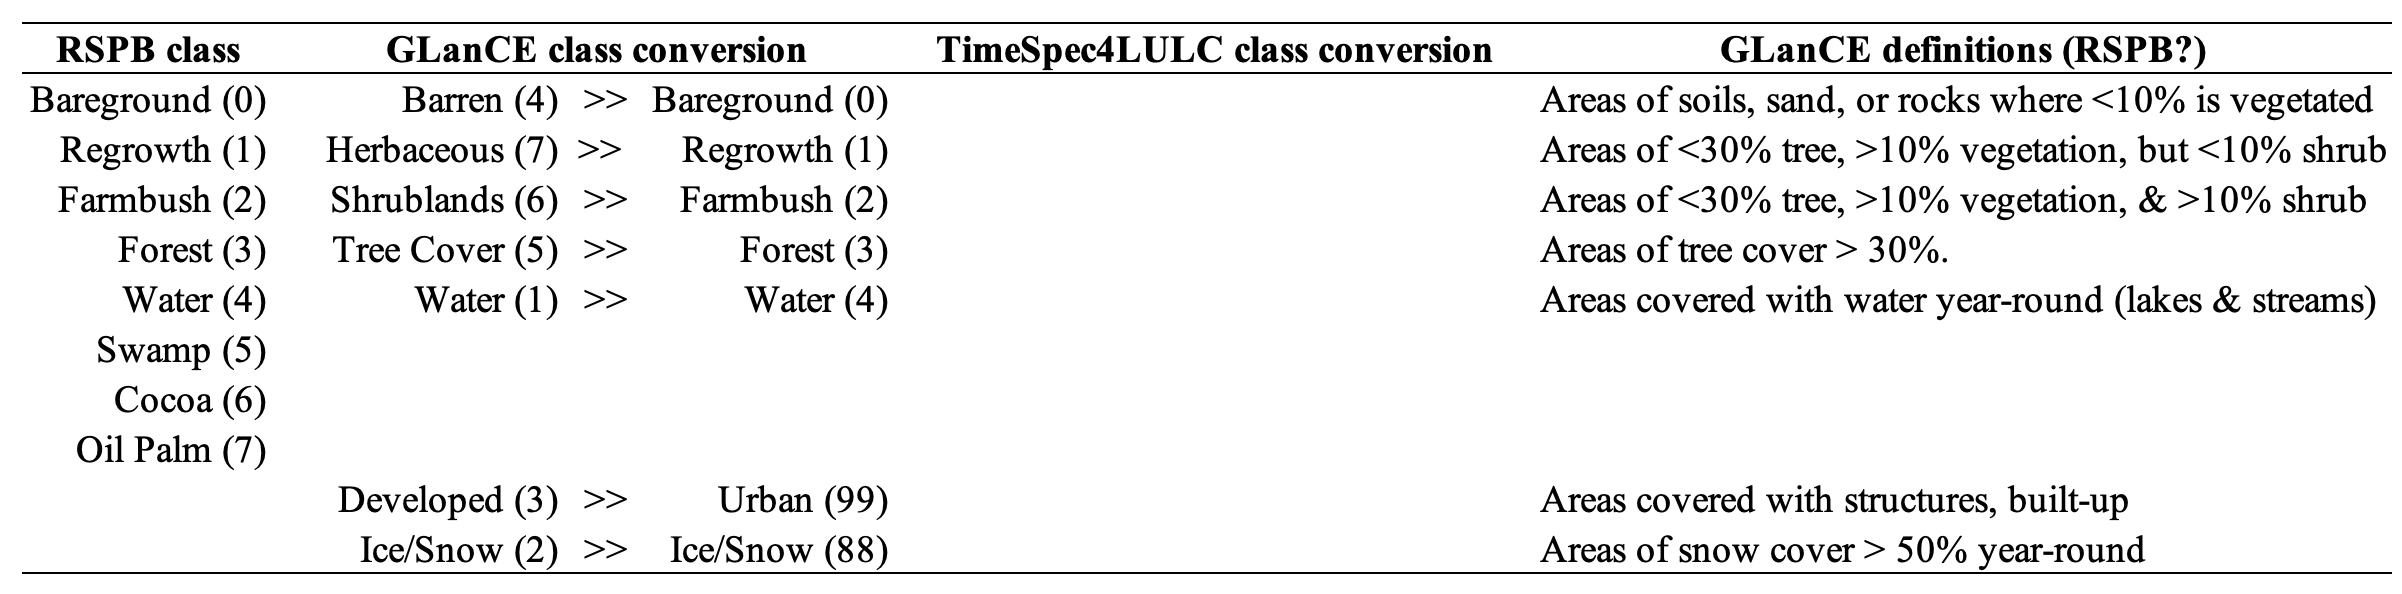
\includegraphics[keepaspectratio]{images/Table 2 Training samples class conversions.png}}

\subparagraph{Table 3: Class conversions of training
samples}\label{table-3-class-conversions-of-training-samples}

Level-1 classes in the GLanCE and TimeSpec4LULC datasets were recoded
below to match class labels cited in the ``Lookups'' sheet of
``ER\_Workbook\_Gola\_Liberia.xlsx'', and the report titled ``Liberia's
Forest Reference Emission Level Submission to the UNFCCC (Woodcock et
al., n.d.; Liberia 2019).

\begin{Shaded}
\begin{Highlighting}[]
\CommentTok{\# import \& tidy samples}
\NormalTok{samples\_raw }\OtherTok{=} \FunctionTok{read.csv}\NormalTok{(}\StringTok{"./data/training\_samples/glance\_training.csv"}\NormalTok{)}
\NormalTok{samples\_clean }\OtherTok{=}\NormalTok{ samples\_raw }\SpecialCharTok{|\textgreater{}}
\NormalTok{  dplyr}\SpecialCharTok{::}\FunctionTok{select}\NormalTok{(Lon, Lat, Glance\_Class\_ID\_level1, Start\_Year, End\_Year)}\SpecialCharTok{|\textgreater{}}
\NormalTok{  dplyr}\SpecialCharTok{::}\FunctionTok{rename}\NormalTok{(}\AttributeTok{longitude =}\NormalTok{ Lon) }\SpecialCharTok{|\textgreater{}}
\NormalTok{  dplyr}\SpecialCharTok{::}\FunctionTok{rename}\NormalTok{(}\AttributeTok{latitude =}\NormalTok{ Lat) }\SpecialCharTok{|\textgreater{}}
\NormalTok{  dplyr}\SpecialCharTok{::}\FunctionTok{rename}\NormalTok{(}\AttributeTok{label\_old =}\NormalTok{ Glance\_Class\_ID\_level1) }\SpecialCharTok{|\textgreater{}}
\NormalTok{  dplyr}\SpecialCharTok{::}\FunctionTok{mutate}\NormalTok{(}\AttributeTok{start\_date =} \FunctionTok{as.Date}\NormalTok{(}\FunctionTok{paste}\NormalTok{(Start\_Year,}\StringTok{"01"}\NormalTok{,}\StringTok{"01"}\NormalTok{,}\AttributeTok{sep =} \StringTok{"{-}"}\NormalTok{)))}\SpecialCharTok{|\textgreater{}}
\NormalTok{  dplyr}\SpecialCharTok{::}\FunctionTok{mutate}\NormalTok{(}\AttributeTok{end\_date =} \FunctionTok{as.Date}\NormalTok{(}\FunctionTok{paste}\NormalTok{(End\_Year, }\StringTok{"01"}\NormalTok{, }\StringTok{"01"}\NormalTok{, }\AttributeTok{sep =} \StringTok{"{-}"}\NormalTok{)))}\SpecialCharTok{|\textgreater{}}
\NormalTok{  dplyr}\SpecialCharTok{::}\FunctionTok{select}\NormalTok{(longitude, latitude, start\_date, end\_date, label\_old)}\SpecialCharTok{|\textgreater{}}
\NormalTok{  dplyr}\SpecialCharTok{::}\FunctionTok{mutate}\NormalTok{(}\AttributeTok{code =} \FunctionTok{case\_when}\NormalTok{(}
\NormalTok{    label\_old }\SpecialCharTok{==} \StringTok{\textquotesingle{}4\textquotesingle{}} \SpecialCharTok{\textasciitilde{}} \DecValTok{0}\NormalTok{, }
\NormalTok{    label\_old }\SpecialCharTok{==} \StringTok{\textquotesingle{}7\textquotesingle{}} \SpecialCharTok{\textasciitilde{}} \DecValTok{1}\NormalTok{, }
\NormalTok{    label\_old }\SpecialCharTok{==} \StringTok{\textquotesingle{}6\textquotesingle{}} \SpecialCharTok{\textasciitilde{}} \DecValTok{2}\NormalTok{, }
\NormalTok{    label\_old }\SpecialCharTok{==} \StringTok{\textquotesingle{}5\textquotesingle{}} \SpecialCharTok{\textasciitilde{}} \DecValTok{3}\NormalTok{, }
\NormalTok{    label\_old }\SpecialCharTok{==} \StringTok{\textquotesingle{}1\textquotesingle{}} \SpecialCharTok{\textasciitilde{}} \DecValTok{4}\NormalTok{, }
\NormalTok{    label\_old }\SpecialCharTok{==} \StringTok{\textquotesingle{}3\textquotesingle{}} \SpecialCharTok{\textasciitilde{}} \DecValTok{99}\NormalTok{, }
\NormalTok{    label\_old }\SpecialCharTok{==} \StringTok{\textquotesingle{}2\textquotesingle{}} \SpecialCharTok{\textasciitilde{}} \DecValTok{88}\NormalTok{)}
\NormalTok{    ) }\SpecialCharTok{|\textgreater{}}
\NormalTok{  dplyr}\SpecialCharTok{::}\FunctionTok{mutate}\NormalTok{(}\AttributeTok{label =} \FunctionTok{case\_when}\NormalTok{(}
\NormalTok{    code }\SpecialCharTok{==} \StringTok{\textquotesingle{}0\textquotesingle{}}  \SpecialCharTok{\textasciitilde{}} \StringTok{"Bareground"}\NormalTok{, }
\NormalTok{    code }\SpecialCharTok{==} \StringTok{\textquotesingle{}1\textquotesingle{}}  \SpecialCharTok{\textasciitilde{}} \StringTok{"Regrowth"}\NormalTok{, }
\NormalTok{    code }\SpecialCharTok{==} \StringTok{\textquotesingle{}2\textquotesingle{}}  \SpecialCharTok{\textasciitilde{}} \StringTok{"Farmbush"}\NormalTok{, }
\NormalTok{    code }\SpecialCharTok{==} \StringTok{\textquotesingle{}3\textquotesingle{}}  \SpecialCharTok{\textasciitilde{}} \StringTok{"TreeCover"}\NormalTok{, }
\NormalTok{    code }\SpecialCharTok{==} \StringTok{\textquotesingle{}4\textquotesingle{}}  \SpecialCharTok{\textasciitilde{}} \StringTok{"Water"}\NormalTok{, }
\NormalTok{    code }\SpecialCharTok{==} \StringTok{\textquotesingle{}99\textquotesingle{}} \SpecialCharTok{\textasciitilde{}} \StringTok{"Urban"}\NormalTok{, }
\NormalTok{    code }\SpecialCharTok{==} \StringTok{\textquotesingle{}88\textquotesingle{}} \SpecialCharTok{\textasciitilde{}} \StringTok{"Snow"}\NormalTok{)}
\NormalTok{    ) }\SpecialCharTok{|\textgreater{}} 
\NormalTok{  dplyr}\SpecialCharTok{::}\FunctionTok{mutate}\NormalTok{(}\AttributeTok{label =} \FunctionTok{as.factor}\NormalTok{(label)) }\SpecialCharTok{|\textgreater{}}
\NormalTok{  dplyr}\SpecialCharTok{::}\FunctionTok{mutate}\NormalTok{(}\AttributeTok{id =} \FunctionTok{row\_number}\NormalTok{()) }\SpecialCharTok{|\textgreater{}} 
\NormalTok{  dplyr}\SpecialCharTok{::}\FunctionTok{select}\NormalTok{(}\SpecialCharTok{{-}}\NormalTok{label\_old) }\SpecialCharTok{|\textgreater{}}
\NormalTok{  dplyr}\SpecialCharTok{::}\FunctionTok{select}\NormalTok{(}\SpecialCharTok{{-}}\NormalTok{code)}
\CommentTok{\# filter to project}
\NormalTok{samples\_sf       }\OtherTok{=}\NormalTok{ sf}\SpecialCharTok{::}\FunctionTok{st\_as\_sf}\NormalTok{(samples\_clean, }\AttributeTok{crs =} \DecValTok{4326}\NormalTok{, }\AttributeTok{coords =} \FunctionTok{c}\NormalTok{(}\StringTok{"longitude"}\NormalTok{, }\StringTok{"latitude"}\NormalTok{))}
\NormalTok{samples\_clipped  }\OtherTok{=}\NormalTok{ sf}\SpecialCharTok{::}\FunctionTok{st\_intersection}\NormalTok{(samples\_sf, country) }\CommentTok{\# n = 364}
\NormalTok{samples\_country  }\OtherTok{=}\NormalTok{ samples\_sf[samples\_clipped, ] }\SpecialCharTok{|\textgreater{}}\NormalTok{ sf}\SpecialCharTok{::}\FunctionTok{st\_transform}\NormalTok{(}\DecValTok{4326}\NormalTok{)}
\NormalTok{samples          }\OtherTok{=}\NormalTok{ sf}\SpecialCharTok{::}\FunctionTok{st\_crop}\NormalTok{(samples\_country, }\FunctionTok{st\_bbox}\NormalTok{(country))}
\NormalTok{sf}\SpecialCharTok{::}\FunctionTok{st\_write}\NormalTok{(samples, }\StringTok{"./data/training\_samples/glance\_spatial\_clip.shp"}\NormalTok{, }\AttributeTok{delete\_dsn =}\NormalTok{ T)}
\FunctionTok{write.csv}\NormalTok{(samples, }\StringTok{"./data/training\_samples/glance\_spatial\_clip.csv"}\NormalTok{, }\AttributeTok{row.names =}\NormalTok{ F)}
\NormalTok{dplyr}\SpecialCharTok{::}\FunctionTok{count}\NormalTok{(samples, label)}
\end{Highlighting}
\end{Shaded}

\begin{verbatim}
Reading layer `glance_spatial_clip' from data source 
  `/Users/seamus/repos/rspb-redd-feasability/data/training_samples/glance_spatial_clip.shp' 
  using driver `ESRI Shapefile'
Simple feature collection with 364 features and 5 fields
Geometry type: POINT
Dimension:     XY
Bounding box:  xmin: -11.41444 ymin: 4.608361 xmax: -7.579165 ymax: 8.353939
Geodetic CRS:  WGS 84
\end{verbatim}

\begin{longtable}[]{@{}lrl@{}}
\toprule\noalign{}
label & n & geometry \\
\midrule\noalign{}
\endhead
\bottomrule\noalign{}
\endlastfoot
Farmbush & 4 & MULTIPOINT ((-11.35816 6.81\ldots{} \\
Regrowth & 9 & MULTIPOINT ((-9.780878 6.16\ldots{} \\
TreeCover & 311 & MULTIPOINT ((-11.41444 6.96\ldots{} \\
Urban & 37 & MULTIPOINT ((-10.78342 6.36\ldots{} \\
Water & 3 & MULTIPOINT ((-11.26555 6.76\ldots{} \\
\end{longtable}

\textbf{\emph{Raster collection}}

The dataset of STAC-formatted Landsat Collection-2-Level-2 was extracted
from the Google Earth Engine Catalog and processed using a cloudless and
pixel quality ranking mask before back-filling with median
normalization. This was implemented in a
\href{https://drive.google.com/file/d/1Vn0KDzkFDaBhpdC803IbYVRuu5cHx0SO/view?usp=drive_link}{Colab
python runtime here}. The collection of unclassified raster outputs was
temporarily stored in
\href{https://drive.google.com/drive/folders/1XMYYhBUAsvuZ02avsZHYHDTArqztLaFI?usp=drive_link}{Google
Drive folder} and the consolidated, resampled and labelled full stack
was stored
\href{https://drive.google.com/file/d/1Vn0KDzkFDaBhpdC803IbYVRuu5cHx0SO/view?usp=drive_link}{here}.

Landsat data was acquired instead of Sentinel imagery due to start date
of project's 10-year baseline occurring before the launch of the
Sentinel 2 satellite. The following chunk provides an alternative
worflow, though less reliable, R-native workflow for acquiring,
aligning, and processing rasters for the extent of Liberia.

\begin{Shaded}
\begin{Highlighting}[]
\NormalTok{roi }\OtherTok{\textless{}{-}} \FunctionTok{st\_bbox}\NormalTok{(country) }\SpecialCharTok{\%\textgreater{}\%} \FunctionTok{st\_as\_sfc}\NormalTok{()}
\CommentTok{\# cube assembly}
\NormalTok{cube\_2024\_mpc }\OtherTok{\textless{}{-}} \FunctionTok{sits\_cube}\NormalTok{(}
  \AttributeTok{source      =} \StringTok{"MPC"}\NormalTok{,}
  \AttributeTok{collection  =} \StringTok{"LANDSAT{-}C2{-}L2"}\NormalTok{,}
  \AttributeTok{roi         =}\NormalTok{ roi,}
  \AttributeTok{bands       =} \FunctionTok{c}\NormalTok{(}\StringTok{"BLUE"}\NormalTok{, }\StringTok{"GREEN"}\NormalTok{, }\StringTok{"NIR08"}\NormalTok{, }\StringTok{"RED"}\NormalTok{, }\StringTok{"SWIR16"}\NormalTok{, }\StringTok{"SWIR22"}\NormalTok{, }\StringTok{"CLOUD"}\NormalTok{),}
  \AttributeTok{start\_date  =} \StringTok{"2024{-}01{-}01"}\NormalTok{,}
  \AttributeTok{end\_date    =} \StringTok{"2024{-}02{-}01"}
\NormalTok{  )}
\CommentTok{\# cloud{-}mask \& normalization}
\NormalTok{cube\_2024\_reg }\OtherTok{\textless{}{-}} \FunctionTok{sits\_regularize}\NormalTok{(}
  \AttributeTok{cube        =}\NormalTok{ cube\_2024\_mpc,}
  \AttributeTok{res         =} \DecValTok{30}\NormalTok{,}
  \AttributeTok{period      =} \StringTok{"P60D"}\NormalTok{,}
  \AttributeTok{multicores  =} \DecValTok{16}\NormalTok{,}
  \AttributeTok{output\_dir  =} \StringTok{"./data/cube\_stac"}\NormalTok{)}
\CommentTok{\# Derive NDVI}
\NormalTok{cube\_2024\_spectral }\OtherTok{=}\NormalTok{ sits}\SpecialCharTok{::}\FunctionTok{sits\_apply}\NormalTok{(}
  \AttributeTok{data        =}\NormalTok{ cube\_2024\_reg,}
  \AttributeTok{NDVI        =}\NormalTok{ (NIR08 }\SpecialCharTok{{-}}\NormalTok{ RED) }\SpecialCharTok{/}\NormalTok{ (NIR08 }\SpecialCharTok{+}\NormalTok{ RED), }
  \AttributeTok{output\_dir  =} \StringTok{"./data/cube\_stac"}\NormalTok{,}
  \AttributeTok{memsize     =} \DecValTok{8}\NormalTok{,}
  \AttributeTok{multicores  =} \DecValTok{16}\NormalTok{,}
  \AttributeTok{progress    =}\NormalTok{ T}
\NormalTok{  )}
\CommentTok{\# Sequence of raster stack}
\NormalTok{STACK }\OtherTok{=} \FunctionTok{brick}\NormalTok{(NDVI\_2014, NDVI\_2019, NDVI\_2024,}
\NormalTok{          BLUE\_2014, BLUE\_2019, BLUE\_2024, }
\NormalTok{          GREEN\_2014, GREEN\_2019, GREEN\_2024,}
\NormalTok{          NIR08\_2014, NIR08\_2019, NIR08\_2024, }
\NormalTok{          RED\_2014, RED\_2019, RED\_2024, }
\NormalTok{          SWIR16\_2014, SWIR16\_2019, SWIR16\_2024, }
\NormalTok{          SWIR22\_2014, SWIR22\_2019, SWIR22\_2024,}
\NormalTok{          DEM)}
\end{Highlighting}
\end{Shaded}

The processes above were repeated for three baseline years of 2014,
2019, and 2024, which were then saved as raster stacked and visualized
below.

\begin{Shaded}
\begin{Highlighting}[]
\CommentTok{\# import}
\NormalTok{NDVI\_2014}\OtherTok{=}\NormalTok{terra}\SpecialCharTok{::}\FunctionTok{rast}\NormalTok{(}\StringTok{"\textasciitilde{}/repos/rspb{-}redd{-}feasability/data/STACK/LANDSAT\_TM{-}ETM{-}OLI\_198055\_NDVI\_2014{-}01{-}04.tif"}\NormalTok{)}
\NormalTok{NDVI\_2019}\OtherTok{=}\NormalTok{terra}\SpecialCharTok{::}\FunctionTok{rast}\NormalTok{(}\StringTok{"\textasciitilde{}/repos/rspb{-}redd{-}feasability/data/STACK/LANDSAT\_TM{-}ETM{-}OLI\_198055\_NDVI\_2019{-}01{-}02.tif"}\NormalTok{)}
\NormalTok{NDVI\_2024}\OtherTok{=}\NormalTok{terra}\SpecialCharTok{::}\FunctionTok{rast}\NormalTok{(}\StringTok{"\textasciitilde{}/repos/rspb{-}redd{-}feasability/data/STACK/LANDSAT\_TM{-}ETM{-}OLI\_198055\_NDVI\_2024{-}01{-}16.tif"}\NormalTok{)}
\NormalTok{STACK}\OtherTok{=}\NormalTok{raster}\SpecialCharTok{::}\FunctionTok{brick}\NormalTok{(}
  \StringTok{"\textasciitilde{}/repos/rspb{-}redd{-}feasability/data/STACK/LANDSAT\_TM{-}ETM{-}OLI\_198055\_STACK{-}\&{-}DEM\_2014{-}01{-}04\_2024{-}01{-}16.tif"}\NormalTok{)}

\CommentTok{\# visualize}
\FunctionTok{hist}\NormalTok{(NDVI\_2014, }\AttributeTok{main =} \StringTok{"NDVI Distribution, 2014"}\NormalTok{, }\AttributeTok{col =} \StringTok{"springgreen"}\NormalTok{) }
\FunctionTok{hist}\NormalTok{(NDVI\_2019, }\AttributeTok{main =} \StringTok{"NDVI Distribution, 2019"}\NormalTok{, }\AttributeTok{col =} \StringTok{"springgreen"}\NormalTok{)}
\FunctionTok{hist}\NormalTok{(NDVI\_2024, }\AttributeTok{main =} \StringTok{"NDVI Distribution, 2024"}\NormalTok{, }\AttributeTok{col =} \StringTok{"springgreen"}\NormalTok{)}
\FunctionTok{plot}\NormalTok{(NDVI\_2014,}\AttributeTok{main=}\StringTok{"NDVI, 2014"}\NormalTok{,}\AttributeTok{xlim=}\FunctionTok{c}\NormalTok{(}\SpecialCharTok{{-}}\FloatTok{11.5}\NormalTok{,}\SpecialCharTok{{-}}\FloatTok{7.5}\NormalTok{),}\AttributeTok{ylim=}\FunctionTok{c}\NormalTok{(}\FloatTok{4.1}\NormalTok{,}\FloatTok{8.6}\NormalTok{),}\AttributeTok{border=}\StringTok{"gray"}\NormalTok{)}
\FunctionTok{plot}\NormalTok{(}\FunctionTok{st\_geometry}\NormalTok{(samples), }\AttributeTok{add=}\NormalTok{T)}
\FunctionTok{plot}\NormalTok{(NDVI\_2019,}\AttributeTok{main=}\StringTok{"NDVI, 2014"}\NormalTok{,}\AttributeTok{xlim=}\FunctionTok{c}\NormalTok{(}\SpecialCharTok{{-}}\FloatTok{11.5}\NormalTok{,}\SpecialCharTok{{-}}\FloatTok{7.5}\NormalTok{),}\AttributeTok{ylim=}\FunctionTok{c}\NormalTok{(}\FloatTok{4.1}\NormalTok{,}\FloatTok{8.6}\NormalTok{),}\AttributeTok{border=}\StringTok{"gray"}\NormalTok{)}
\FunctionTok{plot}\NormalTok{(}\FunctionTok{st\_geometry}\NormalTok{(samples), }\AttributeTok{add=}\NormalTok{T)}
\FunctionTok{plot}\NormalTok{(NDVI\_2024,}\AttributeTok{main=}\StringTok{"NDVI, 2014"}\NormalTok{,}\AttributeTok{xlim=}\FunctionTok{c}\NormalTok{(}\SpecialCharTok{{-}}\FloatTok{11.5}\NormalTok{,}\SpecialCharTok{{-}}\FloatTok{7.5}\NormalTok{),}\AttributeTok{ylim=}\FunctionTok{c}\NormalTok{(}\FloatTok{4.1}\NormalTok{,}\FloatTok{8.6}\NormalTok{),}\AttributeTok{border=}\StringTok{"gray"}\NormalTok{)}
\FunctionTok{plot}\NormalTok{(}\FunctionTok{st\_geometry}\NormalTok{(samples), }\AttributeTok{add=}\NormalTok{T)}
\end{Highlighting}
\end{Shaded}

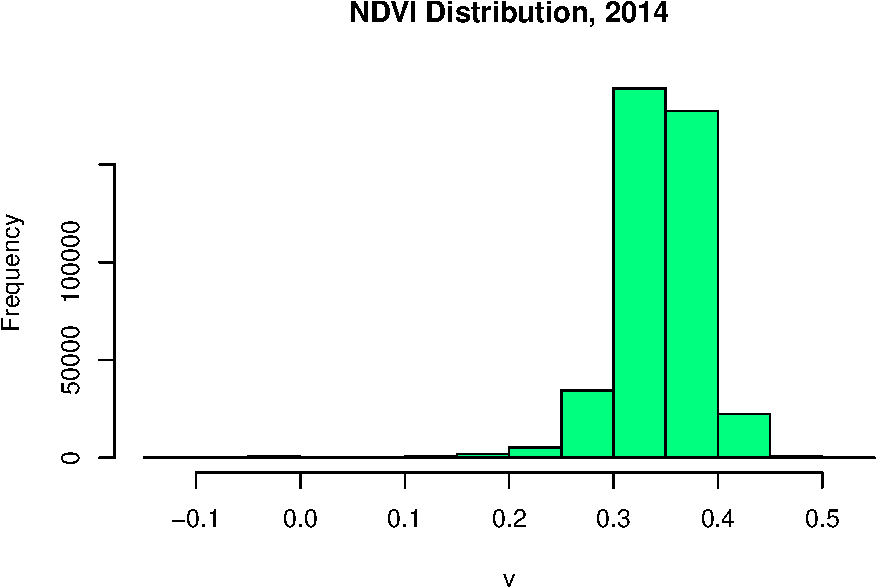
\includegraphics[width=0.33\linewidth]{rspb-gola-redd-review_files/figure-latex/unnamed-chunk-13-1}
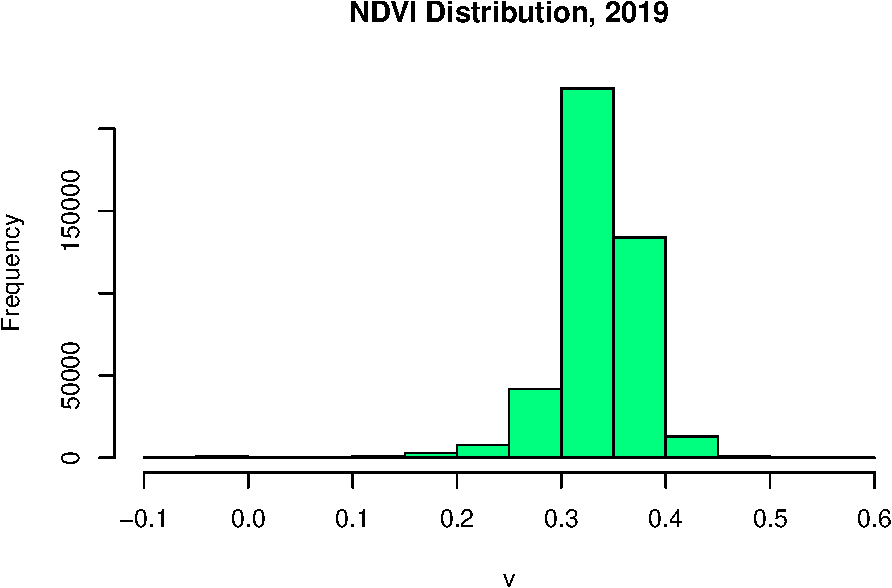
\includegraphics[width=0.33\linewidth]{rspb-gola-redd-review_files/figure-latex/unnamed-chunk-13-2}
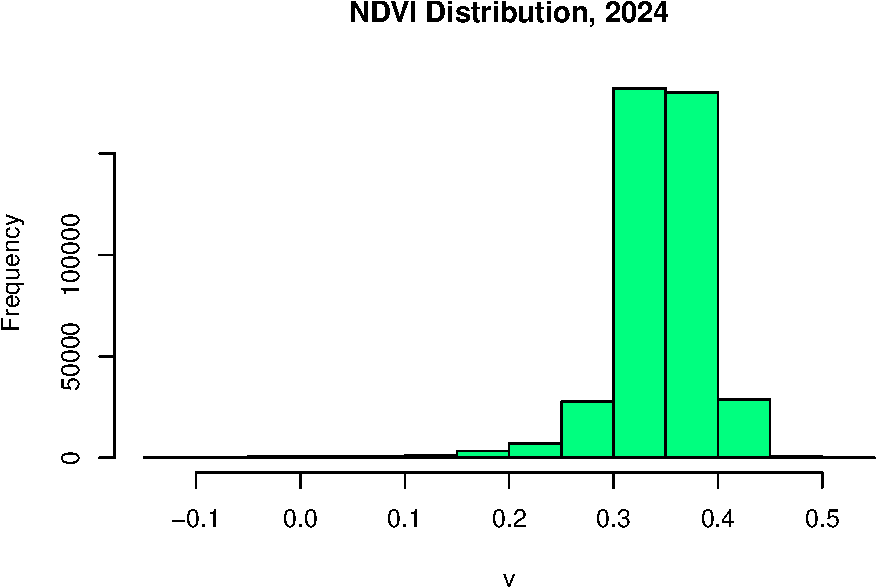
\includegraphics[width=0.33\linewidth]{rspb-gola-redd-review_files/figure-latex/unnamed-chunk-13-3}
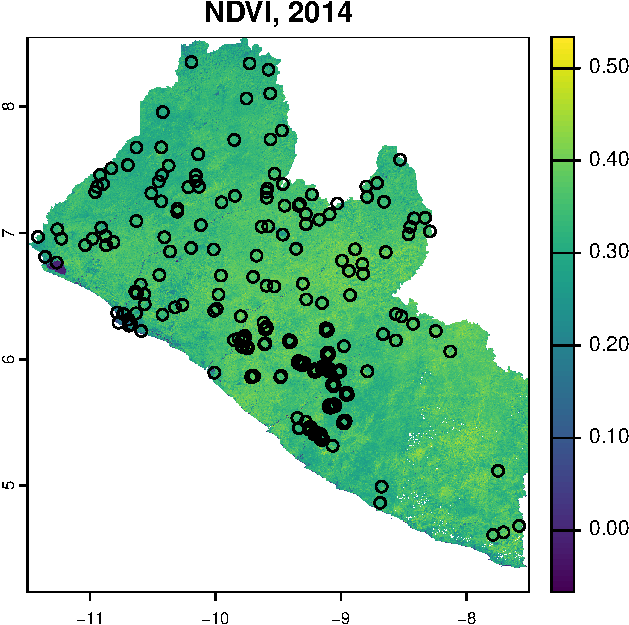
\includegraphics[width=0.33\linewidth]{rspb-gola-redd-review_files/figure-latex/unnamed-chunk-13-4}
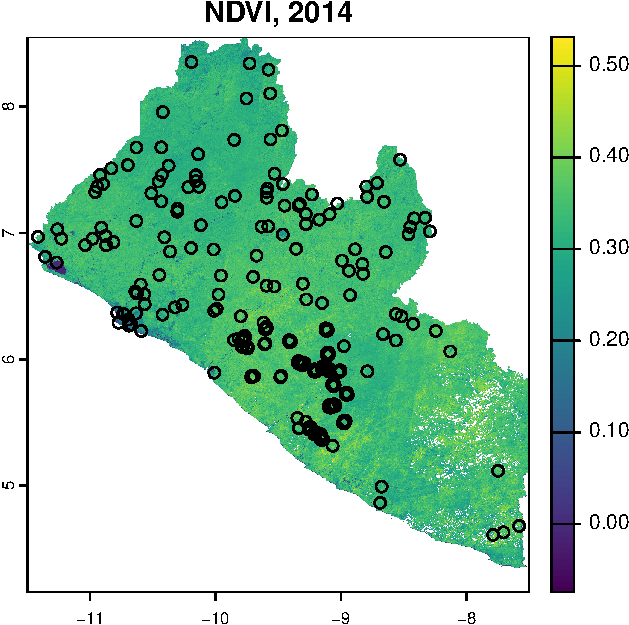
\includegraphics[width=0.33\linewidth]{rspb-gola-redd-review_files/figure-latex/unnamed-chunk-13-5}
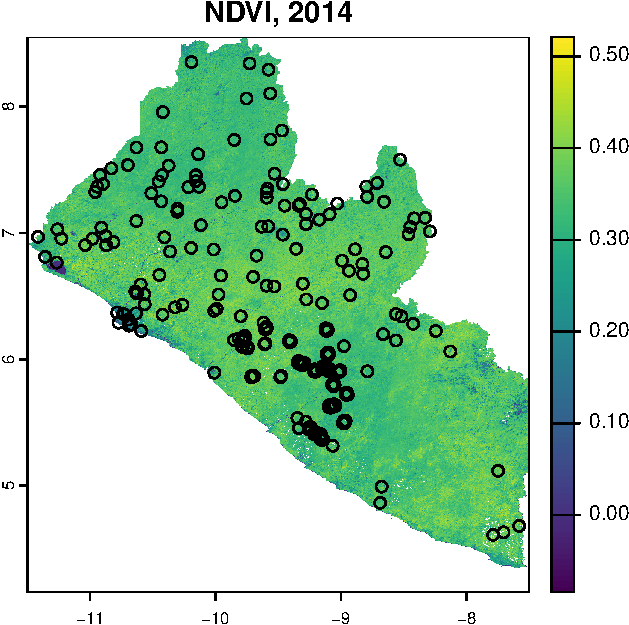
\includegraphics[width=0.33\linewidth]{rspb-gola-redd-review_files/figure-latex/unnamed-chunk-13-6}

\textbf{\emph{Image classification}}

We trained a Random Forest model fitted with 500 decision trees.
Training/test split partitioned the dataset using a 70:30 ratio.
Accuracy assessments were reported using a confusion matrix for full
model and cross-validation estimates. Uncertainty metrics were used to
select best subset of variables according to magnitude and performance.
Models were then calibrated in number regression trees and architecture
rules, with cross-validation reported to assess internal bias from true
population estimates before and to improve uncertainty of final model
deployment.

\begin{Shaded}
\begin{Highlighting}[]
\CommentTok{\# extract yearly layers}
\NormalTok{STACK\_2014}\OtherTok{=}\FunctionTok{subset}\NormalTok{(STACK, }\FunctionTok{c}\NormalTok{(}\StringTok{"NDVI\_2014"}\NormalTok{,}\StringTok{"BLUE\_2014"}\NormalTok{,}\StringTok{"GREEN\_2014"}\NormalTok{,}\StringTok{"NIR08\_2014"}\NormalTok{,}
                           \StringTok{"RED\_2014"}\NormalTok{,}\StringTok{"SWIR16\_2014"}\NormalTok{,}\StringTok{"SWIR22\_2014"}\NormalTok{,}\StringTok{"DEM"}\NormalTok{))}
\CommentTok{\# extract signatures}
\NormalTok{signatures\_2014 }\OtherTok{=}\NormalTok{ raster}\SpecialCharTok{::}\FunctionTok{extract}\NormalTok{(STACK\_2014, samples ,}\AttributeTok{df=}\NormalTok{T) }\CommentTok{\# watch for data formats}
\NormalTok{samples\_signatures\_2014 }\OtherTok{\textless{}{-}}\NormalTok{ dplyr}\SpecialCharTok{::}\FunctionTok{inner\_join}\NormalTok{(signatures\_2014, samples, }\AttributeTok{by=}\FunctionTok{c}\NormalTok{(}\StringTok{"ID"}\OtherTok{=}\StringTok{"id"}\NormalTok{))}
\NormalTok{samples\_signatures\_2014}\SpecialCharTok{$}\NormalTok{geometry }\OtherTok{\textless{}{-}} \ConstantTok{NULL} \CommentTok{\# set geometry to NULL for model training}

\CommentTok{\# training{-}test split, p=0.7 {-}\textgreater{} 70\% split}
\NormalTok{trainIndex\_2014 }\OtherTok{\textless{}{-}}\NormalTok{ caret}\SpecialCharTok{::}\FunctionTok{createDataPartition}\NormalTok{(samples\_signatures\_2014}\SpecialCharTok{$}\NormalTok{ID,}\AttributeTok{list=}\NormalTok{F,}\AttributeTok{p=}\FloatTok{0.7}\NormalTok{)}
\NormalTok{trainData\_2014  }\OtherTok{\textless{}{-}}\NormalTok{ samples\_signatures\_2014[trainIndex\_2014,]  }
\NormalTok{testData\_2014   }\OtherTok{\textless{}{-}}\NormalTok{ samples\_signatures\_2014[}\SpecialCharTok{{-}}\NormalTok{trainIndex\_2014,] }

\CommentTok{\# interpolate NAs with class{-}median{-}normalization (NAs {-}\textgreater{} missing cloud pixels)}
\NormalTok{trainData\_2014 }\OtherTok{\textless{}{-}}\NormalTok{ trainData\_2014 }\SpecialCharTok{|\textgreater{}} \FunctionTok{group\_by}\NormalTok{(label) }\SpecialCharTok{|\textgreater{}} \FunctionTok{mutate}\NormalTok{(}\FunctionTok{across}\NormalTok{(}\FunctionTok{where}\NormalTok{(is.numeric),}
    \SpecialCharTok{\textasciitilde{}} \FunctionTok{ifelse}\NormalTok{(}\FunctionTok{is.na}\NormalTok{(.), }\FunctionTok{median}\NormalTok{(., }\AttributeTok{na.rm =} \ConstantTok{TRUE}\NormalTok{), .))) }\SpecialCharTok{|\textgreater{}} \FunctionTok{ungroup}\NormalTok{()}
\NormalTok{testData\_2014 }\OtherTok{\textless{}{-}}\NormalTok{ testData\_2014 }\SpecialCharTok{|\textgreater{}} \FunctionTok{group\_by}\NormalTok{(label) }\SpecialCharTok{|\textgreater{}} \FunctionTok{mutate}\NormalTok{(}\FunctionTok{across}\NormalTok{(}\FunctionTok{where}\NormalTok{(is.numeric),}
    \SpecialCharTok{\textasciitilde{}} \FunctionTok{ifelse}\NormalTok{(}\FunctionTok{is.na}\NormalTok{(.), }\FunctionTok{median}\NormalTok{(., }\AttributeTok{na.rm =} \ConstantTok{TRUE}\NormalTok{), .))) }\SpecialCharTok{|\textgreater{}} \FunctionTok{ungroup}\NormalTok{()}

\CommentTok{\# assign model variables}
\NormalTok{response  }\OtherTok{\textless{}{-}} \FunctionTok{c}\NormalTok{(}\StringTok{"label"}\NormalTok{)}
\NormalTok{predictors\_2014 }\OtherTok{\textless{}{-}} \FunctionTok{c}\NormalTok{(}
  \StringTok{"NDVI\_2014"}\NormalTok{, }\StringTok{"BLUE\_2014"}\NormalTok{, }\StringTok{"GREEN\_2014"}\NormalTok{, }\StringTok{"RED\_2014"}\NormalTok{, }
  \StringTok{"NIR08\_2014"}\NormalTok{, }\StringTok{"SWIR16\_2014"}\NormalTok{, }\StringTok{"SWIR22\_2014"}\NormalTok{, }\StringTok{"DEM"}
\NormalTok{  )}
\CommentTok{\# set training parameters}
\NormalTok{cv\_regime }\OtherTok{\textless{}{-}}\NormalTok{ caret}\SpecialCharTok{::}\FunctionTok{trainControl}\NormalTok{(}
  \AttributeTok{method          =} \StringTok{\textquotesingle{}cv\textquotesingle{}}\NormalTok{,}
  \AttributeTok{number          =} \DecValTok{10}\NormalTok{,}
  \AttributeTok{savePredictions =}\NormalTok{ T,}
  \AttributeTok{verboseIter     =}\NormalTok{ F}
\NormalTok{  )}

\CommentTok{\# train classifier}
\NormalTok{rf\_model\_2014 }\OtherTok{\textless{}{-}}\NormalTok{ caret}\SpecialCharTok{::}\FunctionTok{train}\NormalTok{(}
\NormalTok{  label}\SpecialCharTok{\textasciitilde{}}\NormalTok{.,}
  \AttributeTok{data =}\NormalTok{ trainData\_2014[, }\FunctionTok{c}\NormalTok{(predictors\_2014, }\StringTok{"label"}\NormalTok{)], }\CommentTok{\# drop ID var}
  \AttributeTok{trControl =}\NormalTok{ cv\_regime,}
  \AttributeTok{method    =} \StringTok{"rf"}\NormalTok{, }
  \AttributeTok{metric    =} \StringTok{\textquotesingle{}Kappa\textquotesingle{}}\NormalTok{, }
  \AttributeTok{ntree     =} \DecValTok{500}\NormalTok{,}
  \AttributeTok{tuneLength=} \DecValTok{6}\NormalTok{,}
  \AttributeTok{importance=}\NormalTok{ T}
\NormalTok{  )}
\end{Highlighting}
\end{Shaded}

\emph{Accuracy assessments (note that randomForest metrics change each
run)}

Results indicated that the model performed well during cross-validation,
achieving a Kappa value of 0.753 and an Accuracy of 94.44\% at an
optimal mtry of 11.

In the blind data test, the model exhibited similar performance,
achieving a Kappa Index of 0.753 and an Accuracy of 94.44\%. This was
accompanied by a No Information Rate (NIR) of 86.11\%, indicating the
model's significant predictive power (ACC = 0.9444, 95\% CI {[}0.883,
0.9793{]}, NIR = 0.8611).

While further investigation is warranted, these results suggest a
moderate concordance between observed and predicted classes. Notably,
key classes such as TreeCover and Urban were predicted with robust
Sensitivity and Specificity (e.g., Forest: SE = 0.9892, SP = 0.7333).

However, the absence of predictions for the `Farmbush' and `Water'
classes points to potential issues with class imbalance or insufficient
representation in the training data. To address these model weaknesses,
we may recommend experimenting with weighted Random Forest or
alternative algorithms such as Gradient Boosting or Support Vector
Machines (SVM) may improve performance for underrepresented classes. The
decision to explore additional modeling strategies is left to the
discretion of project leaders.

\begin{Shaded}
\begin{Highlighting}[]
\NormalTok{rf\_test\_2014 }\OtherTok{\textless{}{-}} \FunctionTok{predict}\NormalTok{(rf\_model\_2014, testData\_2014)}
\FunctionTok{print}\NormalTok{(rf\_model\_2014) }\CommentTok{\# cv results}
\end{Highlighting}
\end{Shaded}

\begin{verbatim}
Random Forest 

256 samples
  8 predictor
  5 classes: 'Farmbush', 'Regrowth', 'TreeCover', 'Urban', 'Water' 

No pre-processing
Resampling: Cross-Validated (10 fold) 
Summary of sample sizes: 231, 230, 229, 231, 229, 231, ... 
Resampling results across tuning parameters:

  mtry  Accuracy   Kappa    
  2     0.9346638  0.7430938
  3     0.9459174  0.7864696
  4     0.9497635  0.7963219
  5     0.9459174  0.7860873
  6     0.9497635  0.7995495
  8     0.9539302  0.8244722

Kappa was used to select the optimal model using the largest value.
The final value used for the model was mtry = 8.
\end{verbatim}

\begin{Shaded}
\begin{Highlighting}[]
\NormalTok{caret}\SpecialCharTok{::}\FunctionTok{confusionMatrix}\NormalTok{(rf\_test\_2014,testData\_2014}\SpecialCharTok{$}\NormalTok{label) }\CommentTok{\# blind test results}
\end{Highlighting}
\end{Shaded}

\begin{verbatim}
Confusion Matrix and Statistics

           Reference
Prediction  Farmbush Regrowth TreeCover Urban Water
  Farmbush         0        0         0     0     0
  Regrowth         0        1         1     0     0
  TreeCover        1        0        92     2     1
  Urban            1        0         0     9     0
  Water            0        0         0     0     0

Overall Statistics
                                         
               Accuracy : 0.9444         
                 95% CI : (0.883, 0.9793)
    No Information Rate : 0.8611         
    P-Value [Acc > NIR] : 0.004895       
                                         
                  Kappa : 0.753          
                                         
 Mcnemar's Test P-Value : NA             

Statistics by Class:

                     Class: Farmbush Class: Regrowth Class: TreeCover
Sensitivity                  0.00000        1.000000           0.9892
Specificity                  1.00000        0.990654           0.7333
Pos Pred Value                   NaN        0.500000           0.9583
Neg Pred Value               0.98148        1.000000           0.9167
Prevalence                   0.01852        0.009259           0.8611
Detection Rate               0.00000        0.009259           0.8519
Detection Prevalence         0.00000        0.018519           0.8889
Balanced Accuracy            0.50000        0.995327           0.8613
                     Class: Urban Class: Water
Sensitivity               0.81818     0.000000
Specificity               0.98969     1.000000
Pos Pred Value            0.90000          NaN
Neg Pred Value            0.97959     0.990741
Prevalence                0.10185     0.009259
Detection Rate            0.08333     0.000000
Detection Prevalence      0.09259     0.000000
Balanced Accuracy         0.90394     0.500000
\end{verbatim}

\emph{Model calibration}

We employed recursive predictor subsetting to identify predictors of
greatest magnitude and non-informative features to enhance model
performance and reduce model complexity, respectively. This aims to
limit potential of multicolinearity, despite inherent robustness of
randomForest algorithms against such violations. The subsetted model was
evaluated on the test dataset. The confusion matrix and performance
metrics were summarized below.

\begin{Shaded}
\begin{Highlighting}[]
\NormalTok{index\_feature\_2014 }\OtherTok{\textless{}{-}} \FunctionTok{createMultiFolds}\NormalTok{(trainData\_2014}\SpecialCharTok{$}\NormalTok{label, }\AttributeTok{times=}\DecValTok{5}\NormalTok{) }
\NormalTok{predictor\_seq\_2014 }\OtherTok{\textless{}{-}}\FunctionTok{seq}\NormalTok{(}\AttributeTok{from=}\DecValTok{1}\NormalTok{, }\AttributeTok{to=}\FunctionTok{length}\NormalTok{(predictors\_2014),}\AttributeTok{by=}\DecValTok{2}\NormalTok{)}

\NormalTok{subset\_regime\_2014 }\OtherTok{\textless{}{-}} \FunctionTok{rfeControl}\NormalTok{(}
  \AttributeTok{method=}\StringTok{"cv"}\NormalTok{,}
  \AttributeTok{number =} \DecValTok{10}\NormalTok{,}
  \AttributeTok{verbose=}\ConstantTok{FALSE}\NormalTok{,}
  \AttributeTok{functions=}\NormalTok{rfFuncs,}
  \AttributeTok{index=}\NormalTok{index\_feature\_2014}
\NormalTok{  )}

\NormalTok{rf\_model\_subset\_2014 }\OtherTok{\textless{}{-}}\NormalTok{ caret}\SpecialCharTok{::}\FunctionTok{rfe}\NormalTok{(}
\NormalTok{  label}\SpecialCharTok{\textasciitilde{}}\NormalTok{.,}
  \AttributeTok{data =}\NormalTok{ trainData\_2014[, }\FunctionTok{c}\NormalTok{(predictors\_2014, }\StringTok{"label"}\NormalTok{)], }
  \AttributeTok{sizes =}\NormalTok{ predictor\_seq\_2014,}
  \AttributeTok{metric =} \StringTok{"Kappa"}\NormalTok{,}
  \AttributeTok{ntree=}\DecValTok{500}\NormalTok{,}
  \AttributeTok{method=}\StringTok{"rf"}\NormalTok{,}
  \AttributeTok{rfeControl =}\NormalTok{ subset\_regime\_2014}
\NormalTok{  )}

\NormalTok{rf\_subset\_test\_2014 }\OtherTok{\textless{}{-}} \FunctionTok{predict}\NormalTok{(rf\_model\_subset\_2014,testData\_2014)}
\FunctionTok{print}\NormalTok{(rf\_model\_subset\_2014)}
\end{Highlighting}
\end{Shaded}

\begin{verbatim}

Recursive feature selection

Outer resampling method: Cross-Validated (10 fold) 

Resampling performance over subset size:

 Variables Accuracy  Kappa AccuracySD KappaSD Selected
         1   0.9026 0.6139    0.04036  0.1539         
         3   0.9448 0.7768    0.04272  0.1792        *
         5   0.9393 0.7552    0.04904  0.1956         
         7   0.9371 0.7470    0.04295  0.1707         
         8   0.9356 0.7408    0.04859  0.1992         

The top 3 variables (out of 3):
   SWIR16_2014, SWIR22_2014, NDVI_2014
\end{verbatim}

\begin{Shaded}
\begin{Highlighting}[]
\NormalTok{caret}\SpecialCharTok{::}\FunctionTok{confusionMatrix}\NormalTok{(rf\_subset\_test\_2014}\SpecialCharTok{$}\NormalTok{pred,testData\_2014}\SpecialCharTok{$}\NormalTok{label)}
\end{Highlighting}
\end{Shaded}

\begin{verbatim}
Confusion Matrix and Statistics

           Reference
Prediction  Farmbush Regrowth TreeCover Urban Water
  Farmbush         0        0         0     0     0
  Regrowth         0        1         1     0     0
  TreeCover        1        0        92     1     0
  Urban            1        0         0    10     0
  Water            0        0         0     0     1

Overall Statistics
                                          
               Accuracy : 0.963           
                 95% CI : (0.9079, 0.9898)
    No Information Rate : 0.8611          
    P-Value [Acc > NIR] : 0.0004509       
                                          
                  Kappa : 0.8456          
                                          
 Mcnemar's Test P-Value : NA              

Statistics by Class:

                     Class: Farmbush Class: Regrowth Class: TreeCover
Sensitivity                  0.00000        1.000000           0.9892
Specificity                  1.00000        0.990654           0.8667
Pos Pred Value                   NaN        0.500000           0.9787
Neg Pred Value               0.98148        1.000000           0.9286
Prevalence                   0.01852        0.009259           0.8611
Detection Rate               0.00000        0.009259           0.8519
Detection Prevalence         0.00000        0.018519           0.8704
Balanced Accuracy            0.50000        0.995327           0.9280
                     Class: Urban Class: Water
Sensitivity               0.90909     1.000000
Specificity               0.98969     1.000000
Pos Pred Value            0.90909     1.000000
Neg Pred Value            0.98969     1.000000
Prevalence                0.10185     0.009259
Detection Rate            0.09259     0.009259
Detection Prevalence      0.10185     0.009259
Balanced Accuracy         0.94939     1.000000
\end{verbatim}

In summary, the subset model achieved an Accuracy of 96.30\% and a Kappa
Index of 0.8456. These metrics closely align with the results of the
original model, suggesting minimal or no loss in predictive power
despite using fewer predictors. Similarly, high-performing classes of
TreeCover and Urban maintained sensitivity and specificity. For example,
TreeCover had a Sensitivity of 0.9892 and Specificity of 0.8667, while
Urban had a Sensitivity of 0.90909 and Specificity of 0.98969. Given
that the reduction in complexity offered by the subsetted model does not
provide significant benefits in this context, we recommend proceeding
with the original model to make spatial predictions.

These modelling operations were repeated for 2019 and 2024 (see Appendix
II).

Spatial predictions were made using their respective models and outputs
of classified LULC rasters were saved in the same Google Drive folder
linked above in previous sections.

\begin{Shaded}
\begin{Highlighting}[]
\CommentTok{\# predict lulc rasters}
\NormalTok{LULC\_LIBERIA\_2014 }\OtherTok{\textless{}{-}}\NormalTok{ raster}\SpecialCharTok{::}\FunctionTok{predict}\NormalTok{(STACK\_2014,rf\_model\_2014) }
\NormalTok{raster}\SpecialCharTok{::}\FunctionTok{writeRaster}\NormalTok{(LULC\_LIBERIA\_2014,}\StringTok{"./data/LULC/LULC\_LIBERIA\_2014{-}01{-}04.tif"}\NormalTok{,}
  \AttributeTok{format =} \StringTok{"GTiff"}\NormalTok{,}\AttributeTok{overwrite =}\NormalTok{ T)}
\NormalTok{LULC\_LIBERIA\_2019 }\OtherTok{\textless{}{-}}\NormalTok{ raster}\SpecialCharTok{::}\FunctionTok{predict}\NormalTok{(STACK\_2019,rf\_model\_2019) }
\NormalTok{raster}\SpecialCharTok{::}\FunctionTok{writeRaster}\NormalTok{(LULC\_LIBERIA\_2019,}\StringTok{"./data/LULC/LULC\_LIBERIA\_2019{-}01{-}02.tif"}\NormalTok{,}
  \AttributeTok{format =} \StringTok{"GTiff"}\NormalTok{,}\AttributeTok{overwrite =}\NormalTok{ T)}
\NormalTok{LULC\_LIBERIA\_2024 }\OtherTok{\textless{}{-}}\NormalTok{ raster}\SpecialCharTok{::}\FunctionTok{predict}\NormalTok{(STACK\_2024,rf\_model\_2024) }
\NormalTok{raster}\SpecialCharTok{::}\FunctionTok{writeRaster}\NormalTok{(LULC\_LIBERIA\_2024,}\StringTok{"./data/LULC/LULC\_LIBERIA\_2024{-}01{-}16.tif"}\NormalTok{,}
  \AttributeTok{format =} \StringTok{"GTiff"}\NormalTok{,}\AttributeTok{overwrite =}\NormalTok{ T)}

\CommentTok{\# visualise}
\NormalTok{LULC\_LIBERIA\_2014 }\OtherTok{=}\NormalTok{ raster}\SpecialCharTok{::}\FunctionTok{raster}\NormalTok{(}\StringTok{"\textasciitilde{}/repos/rspb{-}redd{-}feasability/data/LULC/LULC\_LIBERIA\_2014{-}01{-}04.tif"}\NormalTok{)}
\NormalTok{LULC\_LIBERIA\_2019 }\OtherTok{=}\NormalTok{ raster}\SpecialCharTok{::}\FunctionTok{raster}\NormalTok{(}\StringTok{"\textasciitilde{}/repos/rspb{-}redd{-}feasability/data/LULC/LULC\_LIBERIA\_2019{-}01{-}02.tif"}\NormalTok{)}
\NormalTok{LULC\_LIBERIA\_2024 }\OtherTok{=}\NormalTok{ raster}\SpecialCharTok{::}\FunctionTok{raster}\NormalTok{(}\StringTok{"\textasciitilde{}/repos/rspb{-}redd{-}feasability/data/LULC/LULC\_LIBERIA\_2024{-}01{-}16.tif"}\NormalTok{)}
\NormalTok{terra}\SpecialCharTok{::}\FunctionTok{plot}\NormalTok{(LULC\_LIBERIA\_2014, }\AttributeTok{main=}\StringTok{"Land Cover Classification, 2014"}\NormalTok{)}
\NormalTok{terra}\SpecialCharTok{::}\FunctionTok{plot}\NormalTok{(LULC\_LIBERIA\_2019, }\AttributeTok{main=}\StringTok{"Land Cover Classification, 2019"}\NormalTok{)}
\NormalTok{terra}\SpecialCharTok{::}\FunctionTok{plot}\NormalTok{(LULC\_LIBERIA\_2024, }\AttributeTok{main=}\StringTok{"Land Cover Classification, 2024"}\NormalTok{)}
\end{Highlighting}
\end{Shaded}

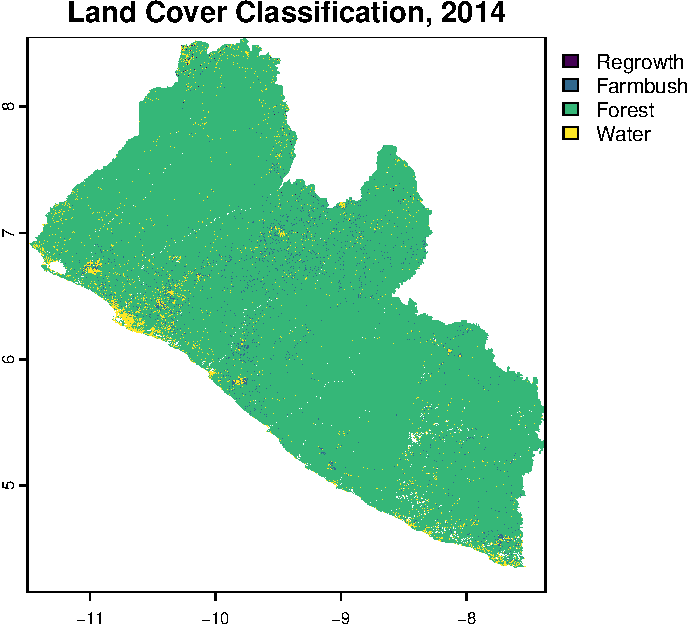
\includegraphics[width=0.33\linewidth]{rspb-gola-redd-review_files/figure-latex/unnamed-chunk-19-1}
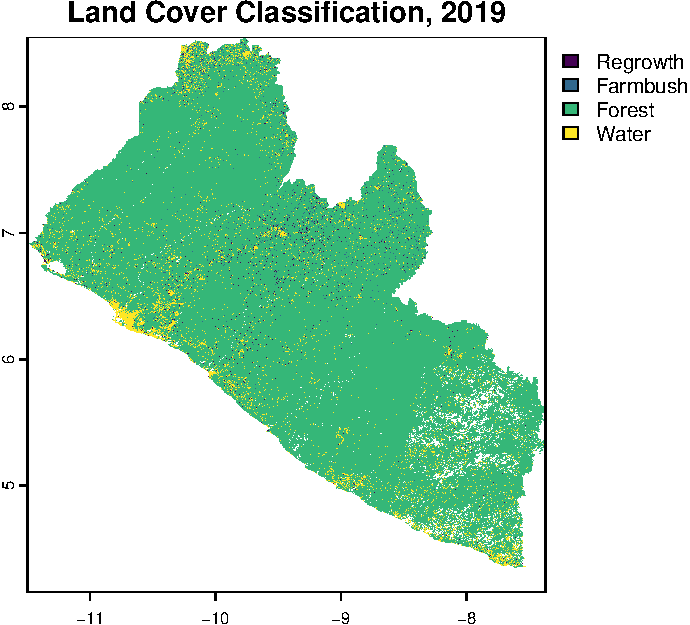
\includegraphics[width=0.33\linewidth]{rspb-gola-redd-review_files/figure-latex/unnamed-chunk-19-2}
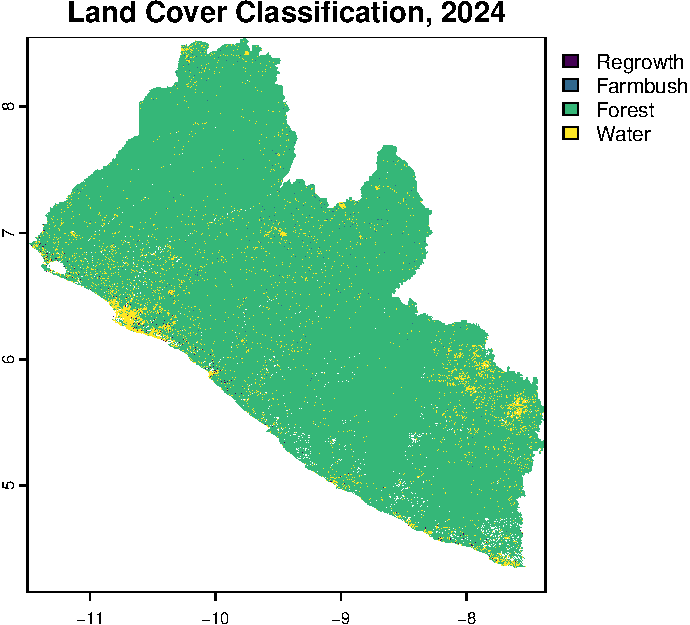
\includegraphics[width=0.33\linewidth]{rspb-gola-redd-review_files/figure-latex/unnamed-chunk-19-3}

\subsubsection{Forest risk maps}\label{forest-risk-maps}

\begin{Shaded}
\begin{Highlighting}[]
\NormalTok{forest\_class }\OtherTok{=} \DecValTok{3}
\NormalTok{forest\_2014 }\OtherTok{\textless{}{-}}\NormalTok{ LULC\_LIBERIA\_2014 }\SpecialCharTok{==}\NormalTok{ forest\_class}
\NormalTok{forest\_2019 }\OtherTok{\textless{}{-}}\NormalTok{ LULC\_LIBERIA\_2019 }\SpecialCharTok{==}\NormalTok{ forest\_class}
\NormalTok{forest\_2024 }\OtherTok{\textless{}{-}}\NormalTok{ LULC\_LIBERIA\_2024 }\SpecialCharTok{==}\NormalTok{ forest\_class}

\NormalTok{terra}\SpecialCharTok{::}\FunctionTok{plot}\NormalTok{(forest\_2014, }\AttributeTok{main=}\StringTok{"Binary Forest Cover Map, 2014"}\NormalTok{)}
\NormalTok{terra}\SpecialCharTok{::}\FunctionTok{plot}\NormalTok{(forest\_2019, }\AttributeTok{main=}\StringTok{"Binary Forest Cover Map, 2019"}\NormalTok{)}
\NormalTok{terra}\SpecialCharTok{::}\FunctionTok{plot}\NormalTok{(forest\_2024, }\AttributeTok{main=}\StringTok{"Binary Forest Cover Map, 2024"}\NormalTok{)}

\CommentTok{\# Forest loss}
\NormalTok{forest\_loss\_2014\_2019 }\OtherTok{\textless{}{-}}\NormalTok{ forest\_2014 }\SpecialCharTok{\&} \SpecialCharTok{!}\NormalTok{forest\_2019}
\NormalTok{forest\_loss\_2019\_2024 }\OtherTok{\textless{}{-}}\NormalTok{ forest\_2019 }\SpecialCharTok{\&} \SpecialCharTok{!}\NormalTok{forest\_2024}
\NormalTok{forest\_loss\_2014\_2024 }\OtherTok{\textless{}{-}}\NormalTok{ forest\_2014 }\SpecialCharTok{\&} \SpecialCharTok{!}\NormalTok{forest\_2024}

\CommentTok{\# Plot forest loss maps}
\NormalTok{terra}\SpecialCharTok{::}\FunctionTok{plot}\NormalTok{(forest\_loss\_2014\_2019, }\AttributeTok{main=}\StringTok{"Forest Loss 2014{-}2019"}\NormalTok{)}
\NormalTok{terra}\SpecialCharTok{::}\FunctionTok{plot}\NormalTok{(forest\_loss\_2019\_2024, }\AttributeTok{main=}\StringTok{"Forest Loss 2019{-}2024"}\NormalTok{)}
\NormalTok{terra}\SpecialCharTok{::}\FunctionTok{plot}\NormalTok{(forest\_loss\_2014\_2024, }\AttributeTok{main=}\StringTok{"Forest Loss 2014{-}2024"}\NormalTok{)}

\CommentTok{\# Save the binary forest maps}
\NormalTok{raster}\SpecialCharTok{::}\FunctionTok{writeRaster}\NormalTok{(forest\_2014, }\StringTok{"\textasciitilde{}/repos/rspb{-}redd{-}feasability/data/LULC/forest\_2014.tif"}\NormalTok{,}\AttributeTok{overwrite=}\NormalTok{T)}
\NormalTok{raster}\SpecialCharTok{::}\FunctionTok{writeRaster}\NormalTok{(forest\_2019, }\StringTok{"\textasciitilde{}/repos/rspb{-}redd{-}feasability/data/LULC/forest\_2019.tif"}\NormalTok{,}\AttributeTok{overwrite=}\NormalTok{T)}
\NormalTok{raster}\SpecialCharTok{::}\FunctionTok{writeRaster}\NormalTok{(forest\_2024, }\StringTok{"\textasciitilde{}/repos/rspb{-}redd{-}feasability/data/LULC/forest\_2024.tif"}\NormalTok{,}\AttributeTok{overwrite=}\NormalTok{T)}

\CommentTok{\# Save the forest loss maps}
\NormalTok{raster}\SpecialCharTok{::}\FunctionTok{writeRaster}\NormalTok{(forest\_loss\_2014\_2019, }\StringTok{"\textasciitilde{}/repos/rspb{-}redd{-}feasability/data/LULC/forest\_loss\_2014\_2019.tif"}\NormalTok{,}\AttributeTok{overwrite=}\NormalTok{T)}
\NormalTok{raster}\SpecialCharTok{::}\FunctionTok{writeRaster}\NormalTok{(forest\_loss\_2019\_2024, }\StringTok{"\textasciitilde{}/repos/rspb{-}redd{-}feasability/data/LULC/forest\_loss\_2019\_2024.tif"}\NormalTok{,}\AttributeTok{overwrite=}\NormalTok{T)}
\NormalTok{raster}\SpecialCharTok{::}\FunctionTok{writeRaster}\NormalTok{(forest\_loss\_2014\_2024, }\StringTok{"\textasciitilde{}/repos/rspb{-}redd{-}feasability/data/LULC/forest\_loss\_2014\_2024.tif"}\NormalTok{,}\AttributeTok{overwrite=}\NormalTok{T)}
\end{Highlighting}
\end{Shaded}

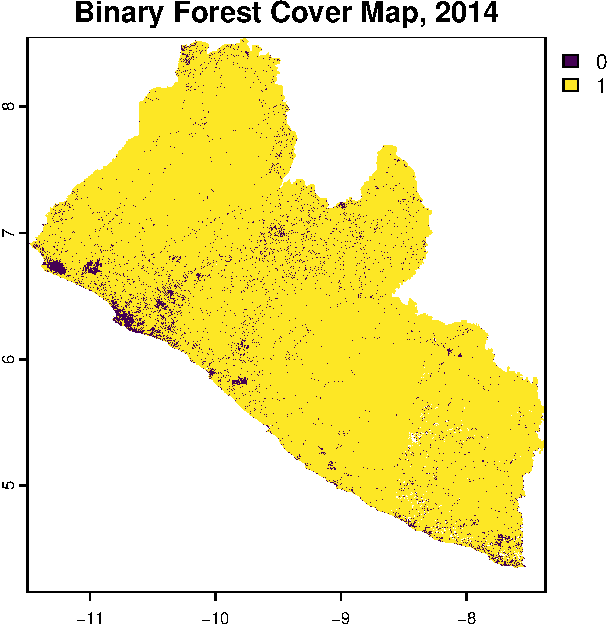
\includegraphics[width=0.33\linewidth]{rspb-gola-redd-review_files/figure-latex/unnamed-chunk-21-1}
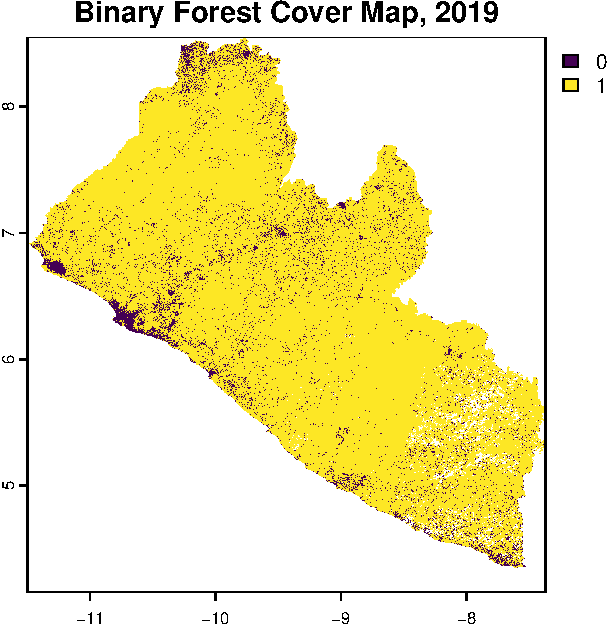
\includegraphics[width=0.33\linewidth]{rspb-gola-redd-review_files/figure-latex/unnamed-chunk-21-2}
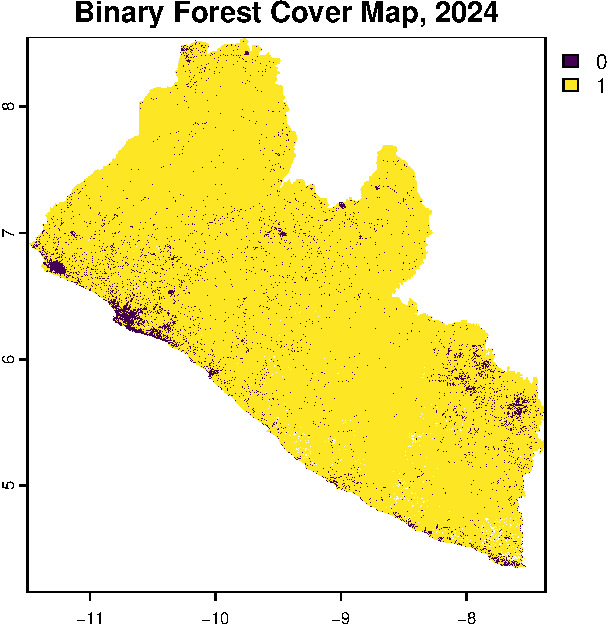
\includegraphics[width=0.33\linewidth]{rspb-gola-redd-review_files/figure-latex/unnamed-chunk-21-3}
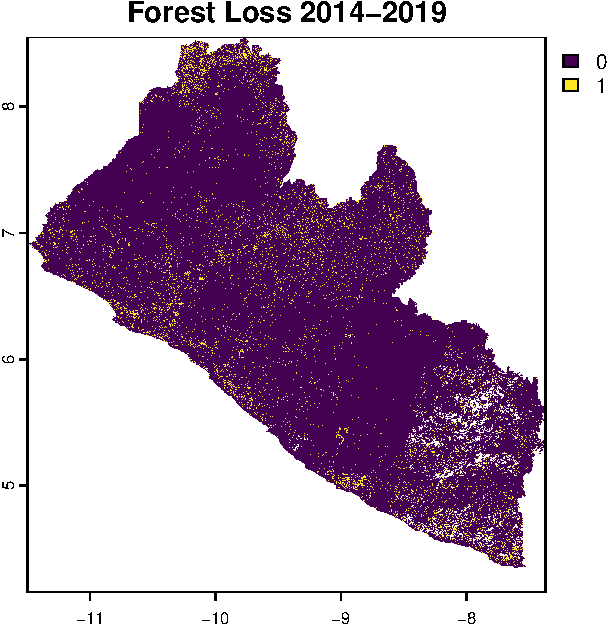
\includegraphics[width=0.33\linewidth]{rspb-gola-redd-review_files/figure-latex/unnamed-chunk-21-4}
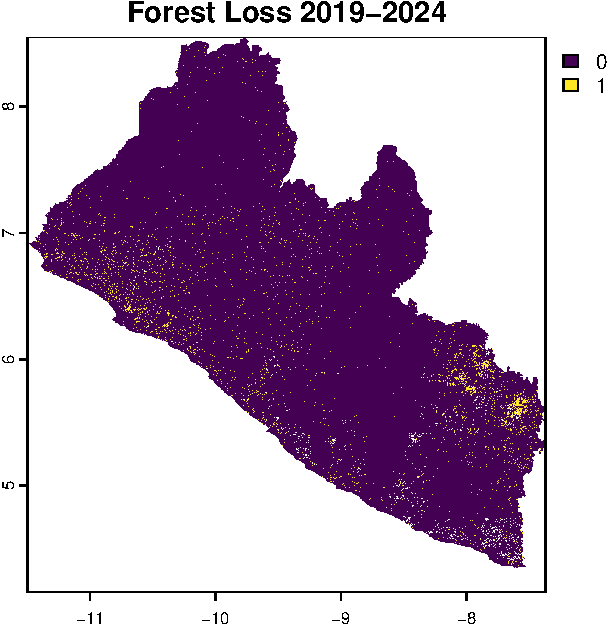
\includegraphics[width=0.33\linewidth]{rspb-gola-redd-review_files/figure-latex/unnamed-chunk-21-5}
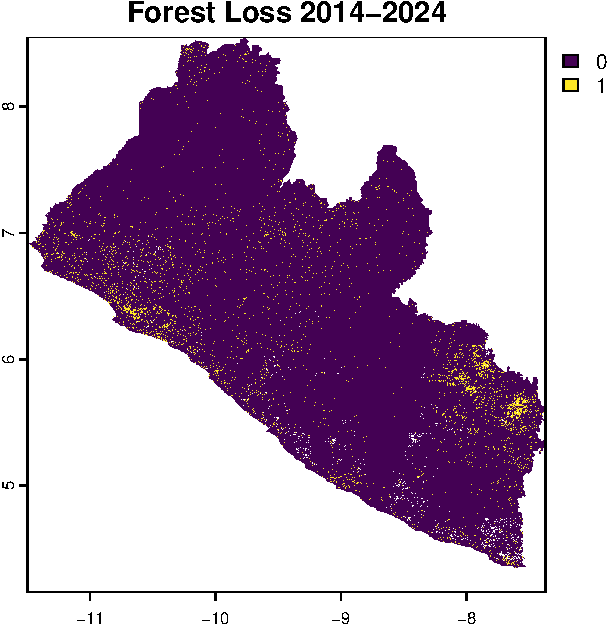
\includegraphics[width=0.33\linewidth]{rspb-gola-redd-review_files/figure-latex/unnamed-chunk-21-6}

\subsubsection{Forest area estimates}\label{forest-area-estimates}

\begin{Shaded}
\begin{Highlighting}[]
\CommentTok{\# reproject to metric estimates}
\NormalTok{forest\_2014 }\OtherTok{\textless{}{-}}\NormalTok{ terra}\SpecialCharTok{::}\FunctionTok{project}\NormalTok{(forest\_2014, }\StringTok{"EPSG:3857"}\NormalTok{)}
\end{Highlighting}
\end{Shaded}

\begin{verbatim}
|---------|---------|---------|---------|=========================================                                          
\end{verbatim}

\begin{Shaded}
\begin{Highlighting}[]
\NormalTok{forest\_2019 }\OtherTok{\textless{}{-}}\NormalTok{ terra}\SpecialCharTok{::}\FunctionTok{project}\NormalTok{(forest\_2019, }\StringTok{"EPSG:3857"}\NormalTok{)}
\end{Highlighting}
\end{Shaded}

\begin{verbatim}
|---------|---------|---------|---------|=========================================                                          
\end{verbatim}

\begin{Shaded}
\begin{Highlighting}[]
\NormalTok{forest\_2024 }\OtherTok{\textless{}{-}}\NormalTok{ terra}\SpecialCharTok{::}\FunctionTok{project}\NormalTok{(forest\_2024, }\StringTok{"EPSG:3857"}\NormalTok{)}
\end{Highlighting}
\end{Shaded}

\begin{verbatim}
|---------|---------|---------|---------|=========================================                                          
\end{verbatim}

\begin{Shaded}
\begin{Highlighting}[]
\CommentTok{\# Calculate total number of forest pixels for each year}
\NormalTok{forest\_pixels\_2014 }\OtherTok{\textless{}{-}} \FunctionTok{sum}\NormalTok{(forest\_2014[], }\AttributeTok{na.rm =} \ConstantTok{TRUE}\NormalTok{)  }
\NormalTok{forest\_pixels\_2019 }\OtherTok{\textless{}{-}} \FunctionTok{sum}\NormalTok{(forest\_2019[], }\AttributeTok{na.rm =} \ConstantTok{TRUE}\NormalTok{)  }
\NormalTok{forest\_pixels\_2024 }\OtherTok{\textless{}{-}} \FunctionTok{sum}\NormalTok{(forest\_2024[], }\AttributeTok{na.rm =} \ConstantTok{TRUE}\NormalTok{)  }

\CommentTok{\# Get the resolution of the raster (assuming square pixels)}
\NormalTok{resolution }\OtherTok{\textless{}{-}} \FunctionTok{res}\NormalTok{(forest\_2014)[}\DecValTok{1}\NormalTok{]}

\CommentTok{\# Calculate the total forest area in square meters}
\NormalTok{forest\_area\_2014 }\OtherTok{\textless{}{-}}\NormalTok{ forest\_pixels\_2014 }\SpecialCharTok{*}\NormalTok{ resolution}\SpecialCharTok{\^{}}\DecValTok{2}
\NormalTok{forest\_area\_2019 }\OtherTok{\textless{}{-}}\NormalTok{ forest\_pixels\_2019 }\SpecialCharTok{*}\NormalTok{ resolution}\SpecialCharTok{\^{}}\DecValTok{2}
\NormalTok{forest\_area\_2024 }\OtherTok{\textless{}{-}}\NormalTok{ forest\_pixels\_2024 }\SpecialCharTok{*}\NormalTok{ resolution}\SpecialCharTok{\^{}}\DecValTok{2}

\CommentTok{\# Convert the total area into hectares (1 hectare = 10,000 square meters)}
\NormalTok{forest\_area\_2014\_ha }\OtherTok{\textless{}{-}}\NormalTok{ forest\_area\_2014 }\SpecialCharTok{/} \DecValTok{10000}
\NormalTok{forest\_area\_2019\_ha }\OtherTok{\textless{}{-}}\NormalTok{ forest\_area\_2019 }\SpecialCharTok{/} \DecValTok{10000}
\NormalTok{forest\_area\_2024\_ha }\OtherTok{\textless{}{-}}\NormalTok{ forest\_area\_2024 }\SpecialCharTok{/} \DecValTok{10000}

\CommentTok{\# Print the results}
\FunctionTok{cat}\NormalTok{(}\StringTok{"Forest area in 2014:"}\NormalTok{, forest\_area\_2014\_ha, }\StringTok{"hectares}\SpecialCharTok{\textbackslash{}n}\StringTok{"}\NormalTok{)}
\end{Highlighting}
\end{Shaded}

\begin{verbatim}
Forest area in 2014: 9332083 hectares
\end{verbatim}

\begin{Shaded}
\begin{Highlighting}[]
\FunctionTok{cat}\NormalTok{(}\StringTok{"Forest area in 2019:"}\NormalTok{, forest\_area\_2019\_ha, }\StringTok{"hectares}\SpecialCharTok{\textbackslash{}n}\StringTok{"}\NormalTok{)}
\end{Highlighting}
\end{Shaded}

\begin{verbatim}
Forest area in 2019: 8851256 hectares
\end{verbatim}

\begin{Shaded}
\begin{Highlighting}[]
\FunctionTok{cat}\NormalTok{(}\StringTok{"Forest area in 2024:"}\NormalTok{, forest\_area\_2024\_ha, }\StringTok{"hectares}\SpecialCharTok{\textbackslash{}n}\StringTok{"}\NormalTok{)}
\end{Highlighting}
\end{Shaded}

\begin{verbatim}
Forest area in 2024: 9297764 hectares
\end{verbatim}

\subsubsection{Benchmarking \&
thresholding}\label{benchmarking-thresholding}

In the following section, we calibrate NDVI thresholds to compare
outputs with unsupervised K-means clustering and the European Space
Agency's Dynamic Global land cover dataset.

\begin{Shaded}
\begin{Highlighting}[]
\CommentTok{\# thresholding}
\NormalTok{ndvi\_float }\OtherTok{=}\NormalTok{ ndvi\_stack }\SpecialCharTok{*} \FloatTok{0.0001}
\NormalTok{ndvi\_thresholds }\OtherTok{\textless{}{-}} \FunctionTok{classify}\NormalTok{(}
\NormalTok{  ndvi\_float, }\FunctionTok{c}\NormalTok{(}\SpecialCharTok{{-}}\FloatTok{1.0}\NormalTok{, }\FloatTok{0.1}\NormalTok{, }\FloatTok{0.4}\NormalTok{, }\FloatTok{0.7}\NormalTok{, }\DecValTok{1}\NormalTok{), }
  \AttributeTok{include.lowest=}\ConstantTok{TRUE}\NormalTok{, }
  \AttributeTok{brackets=}\ConstantTok{TRUE}\NormalTok{)}
\CommentTok{\# kmeans clustering}
\NormalTok{ndvi\_raster }\OtherTok{=}\NormalTok{ raster}\SpecialCharTok{::}\FunctionTok{raster}\NormalTok{(ndvi\_float)}
\NormalTok{nr }\OtherTok{=}\NormalTok{ raster}\SpecialCharTok{::}\FunctionTok{getValues}\NormalTok{(ndvi\_raster)}
\NormalTok{i }\OtherTok{\textless{}{-}} \SpecialCharTok{!}\FunctionTok{is.na}\NormalTok{(nr)}
\NormalTok{kmncluster }\OtherTok{\textless{}{-}} \FunctionTok{kmeans}\NormalTok{(}
\NormalTok{  nr[i], }
  \AttributeTok{centers =} \DecValTok{10}\NormalTok{, }
  \AttributeTok{iter.max =} \DecValTok{500}\NormalTok{, }
  \AttributeTok{nstart =} \DecValTok{5}\NormalTok{, }
  \AttributeTok{algorithm=}\StringTok{"Lloyd"}\NormalTok{)}
\NormalTok{nr[i] }\OtherTok{\textless{}{-}}\NormalTok{ kmncluster}\SpecialCharTok{$}\NormalTok{cluster}
\NormalTok{kmeans }\OtherTok{\textless{}{-}} \FunctionTok{setValues}\NormalTok{(ndvi\_raster, nr)}
\FunctionTok{writeRaster}\NormalTok{(kmeans, }\StringTok{"./data/kmeans/NDVI\_STACK\_KMEANS.tif"}\NormalTok{, }\AttributeTok{overwrite=}\NormalTok{T)}
\FunctionTok{writeRaster}\NormalTok{(ndvi\_thresholds, }\StringTok{"./data/thresholds/NDVI\_STACK\_THRESHOLDS.tif"}\NormalTok{, }\AttributeTok{overwrite=}\NormalTok{T)}
\end{Highlighting}
\end{Shaded}

\subsubsection{Appendix I: 2019 and 2024
classifiers}\label{appendix-i-2019-and-2024-classifiers}

To run these, you may change eval=F to eval=T at the top of chunk in the
.Rmd or .R file saved in the OneDrive folder.

\begin{Shaded}
\begin{Highlighting}[]
\DocumentationTok{\#\#\#\#\#\#\#\#\#\#\#\#\#\#\#\#\#\#\#\#\#\#\#\#\#\#\# 2019}
\CommentTok{\# extract signatures}
\NormalTok{signatures\_2019 }\OtherTok{=}\NormalTok{ raster}\SpecialCharTok{::}\FunctionTok{extract}\NormalTok{(STACK\_2019, samples ,}\AttributeTok{df=}\NormalTok{T) }\CommentTok{\# watch for data formats}
\NormalTok{samples\_signatures\_2019 }\OtherTok{\textless{}{-}}\NormalTok{ dplyr}\SpecialCharTok{::}\FunctionTok{inner\_join}\NormalTok{(signatures\_2019, samples, }\AttributeTok{by=}\FunctionTok{c}\NormalTok{(}\StringTok{"ID"}\OtherTok{=}\StringTok{"id"}\NormalTok{))}
\NormalTok{samples\_signatures\_2019}\SpecialCharTok{$}\NormalTok{geometry }\OtherTok{\textless{}{-}} \ConstantTok{NULL} \CommentTok{\# set geometry to NULL for model training}

\CommentTok{\# training{-}test split, p=0.7 {-}\textgreater{} 70\% split}
\NormalTok{trainIndex\_2019 }\OtherTok{\textless{}{-}}\NormalTok{ caret}\SpecialCharTok{::}\FunctionTok{createDataPartition}\NormalTok{(samples\_signatures\_2019}\SpecialCharTok{$}\NormalTok{ID,}\AttributeTok{list=}\NormalTok{F,}\AttributeTok{p=}\FloatTok{0.7}\NormalTok{)}
\NormalTok{trainData\_2019  }\OtherTok{\textless{}{-}}\NormalTok{ samples\_signatures\_2019[trainIndex\_2019,]  }
\NormalTok{testData\_2019   }\OtherTok{\textless{}{-}}\NormalTok{ samples\_signatures\_2019[}\SpecialCharTok{{-}}\NormalTok{trainIndex\_2019,] }

\CommentTok{\# interpolate NAs with class{-}median{-}normalization (NAs {-}\textgreater{} missing cloud pixels)}
\NormalTok{trainData\_2019 }\OtherTok{\textless{}{-}}\NormalTok{ trainData\_2019 }\SpecialCharTok{|\textgreater{}} \FunctionTok{group\_by}\NormalTok{(label) }\SpecialCharTok{|\textgreater{}} \FunctionTok{mutate}\NormalTok{(}\FunctionTok{across}\NormalTok{(}\FunctionTok{where}\NormalTok{(is.numeric),}
    \SpecialCharTok{\textasciitilde{}} \FunctionTok{ifelse}\NormalTok{(}\FunctionTok{is.na}\NormalTok{(.), }\FunctionTok{median}\NormalTok{(., }\AttributeTok{na.rm =} \ConstantTok{TRUE}\NormalTok{), .))) }\SpecialCharTok{|\textgreater{}} \FunctionTok{ungroup}\NormalTok{()}
\NormalTok{testData\_2019 }\OtherTok{\textless{}{-}}\NormalTok{ testData\_2019 }\SpecialCharTok{|\textgreater{}} \FunctionTok{group\_by}\NormalTok{(label) }\SpecialCharTok{|\textgreater{}} \FunctionTok{mutate}\NormalTok{(}\FunctionTok{across}\NormalTok{(}\FunctionTok{where}\NormalTok{(is.numeric),}
    \SpecialCharTok{\textasciitilde{}} \FunctionTok{ifelse}\NormalTok{(}\FunctionTok{is.na}\NormalTok{(.), }\FunctionTok{median}\NormalTok{(., }\AttributeTok{na.rm =} \ConstantTok{TRUE}\NormalTok{), .))) }\SpecialCharTok{|\textgreater{}} \FunctionTok{ungroup}\NormalTok{()}

\CommentTok{\# assign model variables}
\NormalTok{response  }\OtherTok{\textless{}{-}} \FunctionTok{c}\NormalTok{(}\StringTok{"label"}\NormalTok{)}
\NormalTok{predictors\_2019 }\OtherTok{\textless{}{-}} \FunctionTok{c}\NormalTok{(}
  \StringTok{"NDVI\_2019"}\NormalTok{, }\StringTok{"BLUE\_2019"}\NormalTok{, }\StringTok{"GREEN\_2019"}\NormalTok{, }\StringTok{"RED\_2019"}\NormalTok{, }
  \StringTok{"NIR08\_2019"}\NormalTok{, }\StringTok{"SWIR16\_2019"}\NormalTok{, }\StringTok{"SWIR22\_2019"}\NormalTok{, }\StringTok{"DEM"}
\NormalTok{  )}

\CommentTok{\# train classifier}
\NormalTok{rf\_model\_2019 }\OtherTok{\textless{}{-}}\NormalTok{ caret}\SpecialCharTok{::}\FunctionTok{train}\NormalTok{(}
\NormalTok{  label}\SpecialCharTok{\textasciitilde{}}\NormalTok{.,}
  \AttributeTok{data =}\NormalTok{ trainData\_2019[, }\FunctionTok{c}\NormalTok{(predictors\_2019, }\StringTok{"label"}\NormalTok{)], }\CommentTok{\# drop ID var}
  \AttributeTok{trControl =}\NormalTok{ cv\_regime,}
  \AttributeTok{method    =} \StringTok{"rf"}\NormalTok{, }
  \AttributeTok{metric    =} \StringTok{\textquotesingle{}Kappa\textquotesingle{}}\NormalTok{, }
  \AttributeTok{ntree     =} \DecValTok{500}\NormalTok{,}
  \AttributeTok{tuneLength=} \DecValTok{6}\NormalTok{,}
  \AttributeTok{importance=}\NormalTok{ T}
\NormalTok{  )}

\NormalTok{rf\_test\_2019 }\OtherTok{\textless{}{-}} \FunctionTok{predict}\NormalTok{(rf\_model\_2019, testData\_2019)}
\FunctionTok{print}\NormalTok{(rf\_model\_2019) }\CommentTok{\# cv results}
\FunctionTok{confusionMatrix}\NormalTok{(rf\_test\_2019,testData\_2019}\SpecialCharTok{$}\NormalTok{label) }\CommentTok{\# blind test results}

\NormalTok{index\_feature\_2019 }\OtherTok{\textless{}{-}} \FunctionTok{createMultiFolds}\NormalTok{(trainData\_2019}\SpecialCharTok{$}\NormalTok{label, }\AttributeTok{times=}\DecValTok{5}\NormalTok{) }
\NormalTok{predictor\_seq\_2019 }\OtherTok{\textless{}{-}}\FunctionTok{seq}\NormalTok{(}\AttributeTok{from=}\DecValTok{1}\NormalTok{, }\AttributeTok{to=}\FunctionTok{length}\NormalTok{(predictors\_2019),}\AttributeTok{by=}\DecValTok{2}\NormalTok{)}

\NormalTok{subset\_regime\_2019 }\OtherTok{\textless{}{-}} \FunctionTok{rfeControl}\NormalTok{(}
  \AttributeTok{method=}\StringTok{"cv"}\NormalTok{,}
  \AttributeTok{number =} \DecValTok{10}\NormalTok{,}
  \AttributeTok{verbose=}\ConstantTok{FALSE}\NormalTok{,}
  \AttributeTok{functions=}\NormalTok{rfFuncs,}
  \AttributeTok{index=}\NormalTok{index\_feature\_2019}
\NormalTok{  )}

\NormalTok{rf\_model\_subset\_2019 }\OtherTok{\textless{}{-}}\NormalTok{ caret}\SpecialCharTok{::}\FunctionTok{rfe}\NormalTok{(}
\NormalTok{  label}\SpecialCharTok{\textasciitilde{}}\NormalTok{.,}
  \AttributeTok{data =}\NormalTok{ trainData\_2019[, }\FunctionTok{c}\NormalTok{(predictors\_2019, }\StringTok{"label"}\NormalTok{)], }
  \AttributeTok{sizes =}\NormalTok{ predictor\_seq\_2019,}
  \AttributeTok{metric =} \StringTok{"Kappa"}\NormalTok{,}
  \AttributeTok{ntree=}\DecValTok{500}\NormalTok{,}
  \AttributeTok{method=}\StringTok{"rf"}\NormalTok{,}
  \AttributeTok{rfeControl =}\NormalTok{ subset\_regime\_2019}
\NormalTok{  )}

\NormalTok{rf\_subset\_test\_2019 }\OtherTok{\textless{}{-}} \FunctionTok{predict}\NormalTok{(rf\_model\_subset\_2019,testData\_2019)}
\FunctionTok{print}\NormalTok{(rf\_model\_subset\_2019)}
\FunctionTok{confusionMatrix}\NormalTok{(rf\_subset\_test\_2019}\SpecialCharTok{$}\NormalTok{pred,testData\_2019}\SpecialCharTok{$}\NormalTok{label)}

\DocumentationTok{\#\#\#\#\#\#\#\#\#\#\#\#\#\#\#\#\#\#\#\#\#\#\#\#\# 2024}
\CommentTok{\# extract signatures}
\NormalTok{signatures\_2024 }\OtherTok{=}\NormalTok{ raster}\SpecialCharTok{::}\FunctionTok{extract}\NormalTok{(STACK\_2024, samples ,}\AttributeTok{df=}\NormalTok{T) }\CommentTok{\# watch for data formats}
\NormalTok{samples\_signatures\_2024 }\OtherTok{\textless{}{-}}\NormalTok{ dplyr}\SpecialCharTok{::}\FunctionTok{inner\_join}\NormalTok{(signatures\_2024, samples, }\AttributeTok{by=}\FunctionTok{c}\NormalTok{(}\StringTok{"ID"}\OtherTok{=}\StringTok{"id"}\NormalTok{))}
\NormalTok{samples\_signatures\_2024}\SpecialCharTok{$}\NormalTok{geometry }\OtherTok{\textless{}{-}} \ConstantTok{NULL} \CommentTok{\# set geometry to NULL for model training}

\CommentTok{\# training{-}test split, p=0.7 {-}\textgreater{} 70\% split}
\NormalTok{trainIndex\_2024 }\OtherTok{\textless{}{-}}\NormalTok{ caret}\SpecialCharTok{::}\FunctionTok{createDataPartition}\NormalTok{(samples\_signatures\_2024}\SpecialCharTok{$}\NormalTok{ID,}\AttributeTok{list=}\NormalTok{F,}\AttributeTok{p=}\FloatTok{0.7}\NormalTok{)}
\NormalTok{trainData\_2024  }\OtherTok{\textless{}{-}}\NormalTok{ samples\_signatures\_2024[trainIndex\_2024,]  }
\NormalTok{testData\_2024   }\OtherTok{\textless{}{-}}\NormalTok{ samples\_signatures\_2024[}\SpecialCharTok{{-}}\NormalTok{trainIndex\_2024,] }

\CommentTok{\# interpolate NAs with class{-}median{-}normalization (NAs {-}\textgreater{} missing cloud pixels)}
\NormalTok{trainData\_2024 }\OtherTok{\textless{}{-}}\NormalTok{ trainData\_2024 }\SpecialCharTok{|\textgreater{}} \FunctionTok{group\_by}\NormalTok{(label) }\SpecialCharTok{|\textgreater{}} \FunctionTok{mutate}\NormalTok{(}\FunctionTok{across}\NormalTok{(}\FunctionTok{where}\NormalTok{(is.numeric),}
    \SpecialCharTok{\textasciitilde{}} \FunctionTok{ifelse}\NormalTok{(}\FunctionTok{is.na}\NormalTok{(.), }\FunctionTok{median}\NormalTok{(., }\AttributeTok{na.rm =} \ConstantTok{TRUE}\NormalTok{), .))) }\SpecialCharTok{|\textgreater{}} \FunctionTok{ungroup}\NormalTok{()}
\NormalTok{testData\_2024 }\OtherTok{\textless{}{-}}\NormalTok{ testData\_2024 }\SpecialCharTok{|\textgreater{}} \FunctionTok{group\_by}\NormalTok{(label) }\SpecialCharTok{|\textgreater{}} \FunctionTok{mutate}\NormalTok{(}\FunctionTok{across}\NormalTok{(}\FunctionTok{where}\NormalTok{(is.numeric),}
    \SpecialCharTok{\textasciitilde{}} \FunctionTok{ifelse}\NormalTok{(}\FunctionTok{is.na}\NormalTok{(.), }\FunctionTok{median}\NormalTok{(., }\AttributeTok{na.rm =} \ConstantTok{TRUE}\NormalTok{), .))) }\SpecialCharTok{|\textgreater{}} \FunctionTok{ungroup}\NormalTok{()}
\NormalTok{water\_2014 }\OtherTok{\textless{}{-}}\NormalTok{ trainData\_2014[trainData\_2014}\SpecialCharTok{$}\NormalTok{label }\SpecialCharTok{==} \StringTok{"Water"}\NormalTok{, ]}
\NormalTok{water\_ids }\OtherTok{\textless{}{-}}\NormalTok{ water\_2014}\SpecialCharTok{$}\NormalTok{ID}
\NormalTok{water\_2024 }\OtherTok{\textless{}{-}}\NormalTok{ samples\_signatures\_2024[samples\_signatures\_2024}\SpecialCharTok{$}\NormalTok{ID }\SpecialCharTok{\%in\%}\NormalTok{ water\_ids, ]}
\NormalTok{trainData\_2024 }\OtherTok{\textless{}{-}} \FunctionTok{rbind}\NormalTok{(trainData\_2024, water\_2024)}
\FunctionTok{table}\NormalTok{(trainData\_2024}\SpecialCharTok{$}\NormalTok{label)}

\CommentTok{\# assign model variables}
\NormalTok{response  }\OtherTok{\textless{}{-}} \FunctionTok{c}\NormalTok{(}\StringTok{"label"}\NormalTok{)}
\NormalTok{predictors\_2024 }\OtherTok{\textless{}{-}} \FunctionTok{c}\NormalTok{(}\StringTok{"NDVI\_2024"}\NormalTok{, }\StringTok{"BLUE\_2024"}\NormalTok{, }\StringTok{"GREEN\_2024"}\NormalTok{, }\StringTok{"RED\_2024"}\NormalTok{, }
  \StringTok{"NIR08\_2024"}\NormalTok{, }\StringTok{"SWIR16\_2024"}\NormalTok{, }\StringTok{"SWIR22\_2024"}\NormalTok{, }\StringTok{"DEM"}
\NormalTok{  )}

\CommentTok{\# train classifier}
\NormalTok{rf\_model\_2024 }\OtherTok{\textless{}{-}}\NormalTok{ caret}\SpecialCharTok{::}\FunctionTok{train}\NormalTok{(}
\NormalTok{  label}\SpecialCharTok{\textasciitilde{}}\NormalTok{.,}
  \AttributeTok{data =}\NormalTok{ trainData\_2024[, }\FunctionTok{c}\NormalTok{(predictors\_2024, }\StringTok{"label"}\NormalTok{)], }\CommentTok{\# drop ID var}
  \AttributeTok{trControl =}\NormalTok{ cv\_regime,}
  \AttributeTok{method    =} \StringTok{"rf"}\NormalTok{, }
  \AttributeTok{metric    =} \StringTok{\textquotesingle{}Kappa\textquotesingle{}}\NormalTok{, }
  \AttributeTok{ntree     =} \DecValTok{500}\NormalTok{,}
  \AttributeTok{tuneLength=} \DecValTok{6}\NormalTok{,}
  \AttributeTok{importance=}\NormalTok{ T}
\NormalTok{  )}

\NormalTok{rf\_test\_2024 }\OtherTok{\textless{}{-}} \FunctionTok{predict}\NormalTok{(rf\_model\_2024, testData\_2024)}
\FunctionTok{print}\NormalTok{(rf\_model\_2024) }\CommentTok{\# cv results}
\FunctionTok{confusionMatrix}\NormalTok{(rf\_test\_2024,testData\_2024}\SpecialCharTok{$}\NormalTok{label) }\CommentTok{\# blind test results}

\NormalTok{index\_feature\_2024 }\OtherTok{\textless{}{-}} \FunctionTok{createMultiFolds}\NormalTok{(trainData\_2024}\SpecialCharTok{$}\NormalTok{label, }\AttributeTok{times=}\DecValTok{5}\NormalTok{) }
\NormalTok{predictor\_seq\_2024 }\OtherTok{\textless{}{-}}\FunctionTok{seq}\NormalTok{(}\AttributeTok{from=}\DecValTok{1}\NormalTok{, }\AttributeTok{to=}\FunctionTok{length}\NormalTok{(predictors\_2024),}\AttributeTok{by=}\DecValTok{2}\NormalTok{)}

\NormalTok{subset\_regime\_2024 }\OtherTok{\textless{}{-}} \FunctionTok{rfeControl}\NormalTok{(}
  \AttributeTok{method=}\StringTok{"cv"}\NormalTok{,}
  \AttributeTok{number =} \DecValTok{10}\NormalTok{,}
  \AttributeTok{verbose=}\ConstantTok{FALSE}\NormalTok{,}
  \AttributeTok{functions=}\NormalTok{rfFuncs,}
  \AttributeTok{index=}\NormalTok{index\_feature\_2024}
\NormalTok{  )}

\NormalTok{rf\_model\_subset\_2024 }\OtherTok{\textless{}{-}}\NormalTok{ caret}\SpecialCharTok{::}\FunctionTok{rfe}\NormalTok{(}
\NormalTok{  label}\SpecialCharTok{\textasciitilde{}}\NormalTok{.,}
  \AttributeTok{data =}\NormalTok{ trainData\_2024[, }\FunctionTok{c}\NormalTok{(predictors\_2024, }\StringTok{"label"}\NormalTok{)], }
  \AttributeTok{sizes =}\NormalTok{ predictor\_seq\_2024,}
  \AttributeTok{metric =} \StringTok{"Kappa"}\NormalTok{,}
  \AttributeTok{ntree=}\DecValTok{500}\NormalTok{,}
  \AttributeTok{method=}\StringTok{"rf"}\NormalTok{,}
  \AttributeTok{rfeControl =}\NormalTok{ subset\_regime\_2024}
\NormalTok{  )}

\NormalTok{rf\_subset\_test\_2024 }\OtherTok{\textless{}{-}} \FunctionTok{predict}\NormalTok{(rf\_model\_subset\_2024,testData\_2024)}
\FunctionTok{print}\NormalTok{(rf\_model\_subset\_2024)}
\FunctionTok{confusionMatrix}\NormalTok{(rf\_subset\_test\_2024}\SpecialCharTok{$}\NormalTok{pred,testData\_2024}\SpecialCharTok{$}\NormalTok{label)}
\end{Highlighting}
\end{Shaded}

\phantomsection\label{refs}
\begin{CSLReferences}{1}{0}
\bibitem[\citeproctext]{ref-governmentofliberiaLiberiasForestReference2019}
Liberia, Government of. 2019. \emph{Liberia's Forest Reference Emission
Level Submission to the UNFCCC}. 1. Forestry Development Authority.

\bibitem[\citeproctext]{ref-stanimirovaGlobalLandCover2023}
Stanimirova, Radost, Katelyn Tarrio, Konrad Turlej, Kristina McAvoy,
Sophia Stonebrook, Kai-Ting Hu, Paulo Arévalo, et al. 2023. {``A Global
Land Cover Training Dataset from 1984 to 2020.''} \emph{Scientific Data}
10 (1): 879. \url{https://doi.org/10.1038/s41597-023-02798-5}.

\bibitem[\citeproctext]{ref-verraVT0007UnplannedDeforestation2021}
Verra. 2021. \emph{VT0007: Unplanned Deforestation Allocation Tool}.
0.1. Verra.
\url{https://verra.org/wp-content/uploads/2024/02/VT0007-Unplanned-Deforestation-Allocation-v1.0.pdf}.

\bibitem[\citeproctext]{ref-verraVM0048ReducingEmissions2023a}
---------. 2023. \emph{VM0048: Reducing Emissions from Deforestation and
Forest Degradation}. 1.0. Verra.
\url{https://verra.org/wp-content/uploads/2023/11/VM0048-Reducing-Emissions-from-Deforestation-and-Forest-Degradation-v1.0-1-1.pdf}.

\bibitem[\citeproctext]{ref-verraVMD0055EstimationEmission2024}
---------. 2024. \emph{VMD0055: Estimation of Emission Reductions from
Avoiding Unplanned Deforestation}. VCS Module 1.1. Verra.
\url{https://verra.org/wp-content/uploads/2024/10/VMD0055-Estimation-of-Emission-Reductions-from-Avoiding-Unplanned-Deforestation-v1.1-CLEAN-2024.10.21.24.pdf}.

\bibitem[\citeproctext]{ref-woodcockGlobalLandCover}
Woodcock, Curtis, Pontus Olofsson, Thomas Loveland, Chris Barber, and
Zhe Zhu. n.d. {``Global Land Cover Estimation (GLanCE) Product User
Guide Version 1.0 August 2022.''}

\end{CSLReferences}

\end{document}
